{\bf Problem sheets from Morin -- Introduction to Classical Mechanics}

\section{Strategies for solving problems}
\subsection*{Units \& dimensional analysis}
\subsubsection*{}
\begin{mdframed}
  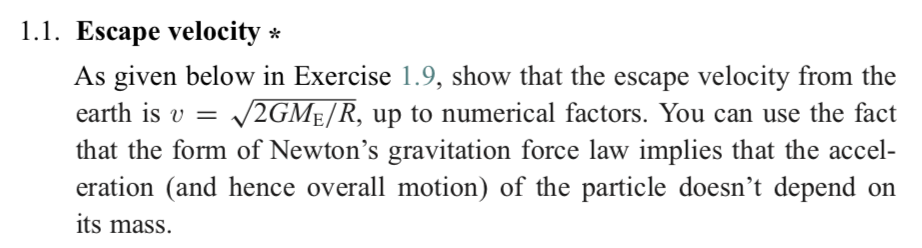
\includegraphics[width=400pt]{img/physics--classical-mechanics--morin--1-1.png}
\end{mdframed}

A projectile of mass $m$ is fired vertically upwards with velocity $v$ (no air-resistance).

When the projectile is at height $h$, the acceleration due to gravity is
$\frac{F}{m} = GM_E/(R + h)^2$, which does not depend on $m$.

We want units of $LT^{-1}$. We have

\begin{tabular*}{1.0\linewidth}{l|l}
  $[G]$        & $L^3M^{-1}T^{-2}$ \\
  $[M_E]$      & $M$ \\
  $[R]$        & $L$ \\
  $[GM_E / R]$ & $L^2T^{-2}$
\end{tabular*}

A quantity with the desired units is $\sqrt{GM_E/R}$.

More formally, suppose $v \propto G^iM_E^jR^k$.

Let  ${G, M_E, R}$ be a basis for a vector space.

Then the problem corresponds to the linear system
\begin{align*}
  \matMMMxNNN
  {3}{0}{1}
  {-1}{1}{0}
  {-2}{0}{0} \vecMMM{i}{j}{k} = \vecMMM{1}{0}{-1}.
\end{align*}
$i$ must be $1/2$, which implies $j = 1/2, k = -1/2$, i.e. $\sqrt{GM_E/R}$. \checkmark

\subsubsection*{}
\begin{mdframed}
  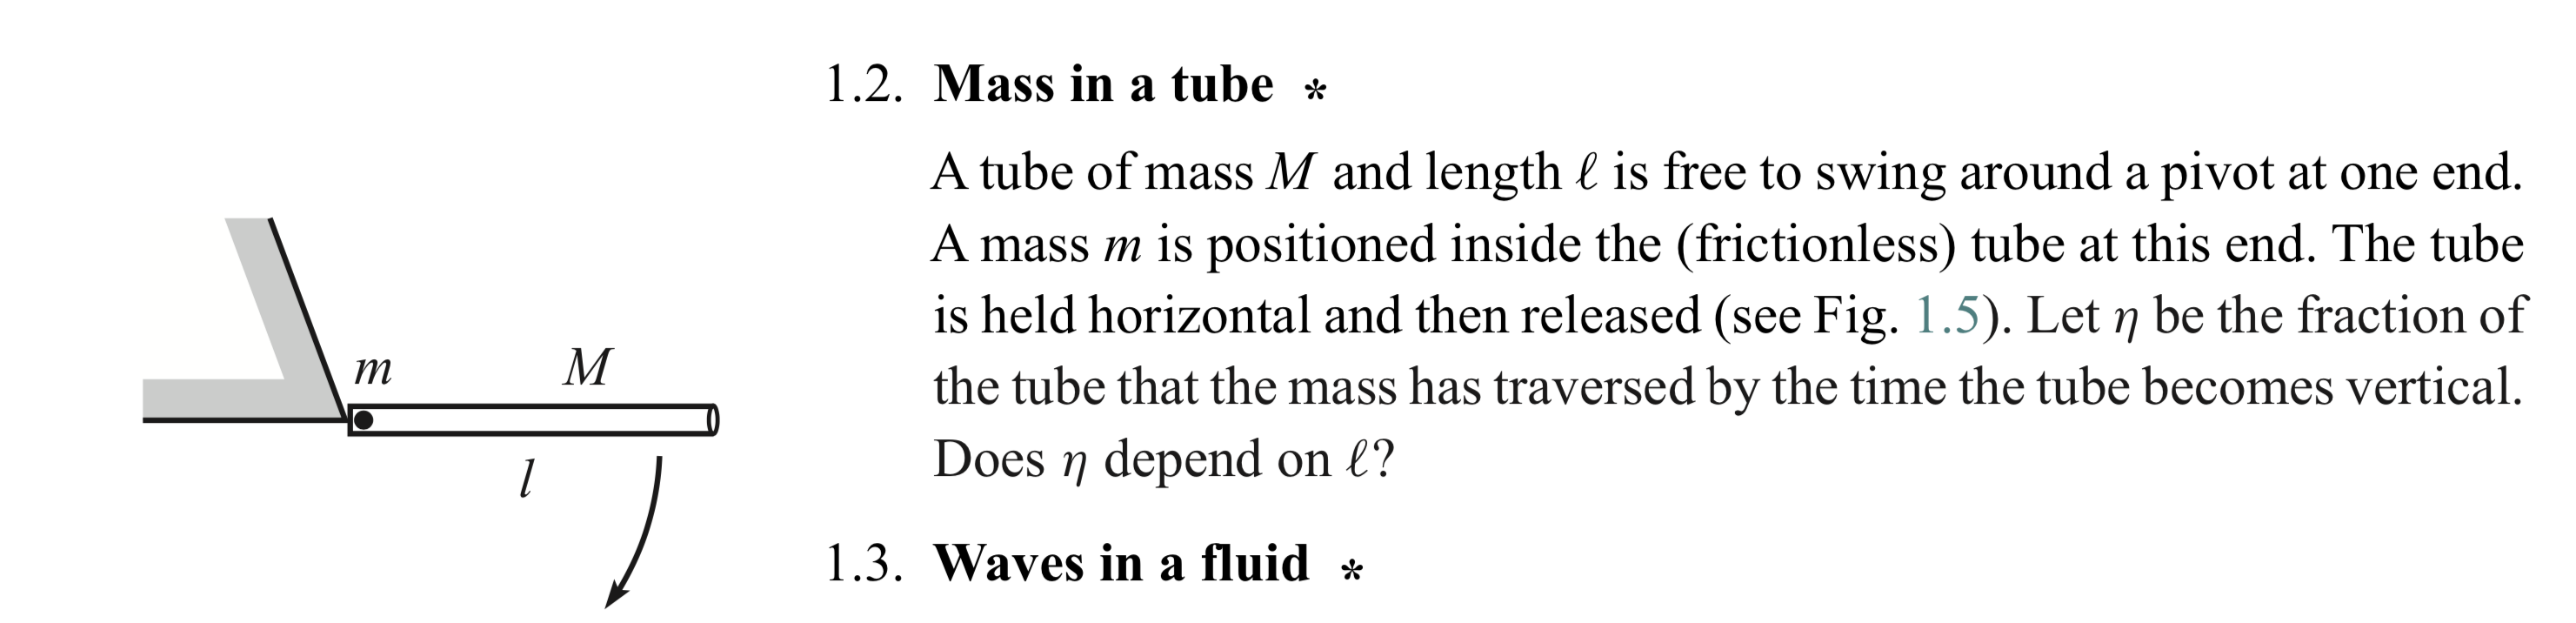
\includegraphics[width=400pt]{img/physics--classical-mechanics--morin--1-2.png}
\end{mdframed}

\begin{enumerate}
\item
  \begin{tabular}{l|l}
    $[l]$       & $L$ \\
    $[m], [M]$  & $M$ \\
    $[g]$       & $LT^{-2}$
  \end{tabular}\\
  As a fraction, $\eta$ is dimensionless. It cannot depend on $g$ since there is no other
  quantity to cancel out the time units. Suppose $\eta$ depends on some power of $l$. Then it must
  also depend on some other quantity involving distance. But there is no other
  such quantity. Therefore $\eta$ does not depend on $l$.  \checkmark

\item \todo{Why is this wrong?} We can choose an $l$ for which $\eta > 0$. Let $\eta^* > 0$ be such
  an $\eta$.

  However, as $l \to \infty$, we have $\eta \to 0$ since the distance traversed by the mass is bounded
  above by the distance the mass would drop under gravity with no opposing normal force from the tube;
  since $m$ is finite, this bound is finite.

  Therefore for all $\eta^* > 0$, we can choose an $l$ such that $\eta < \eta^*$. Therefore $\eta$
  does depend on $l$.
\end{enumerate}

\subsubsection*{}
\begin{mdframed}
  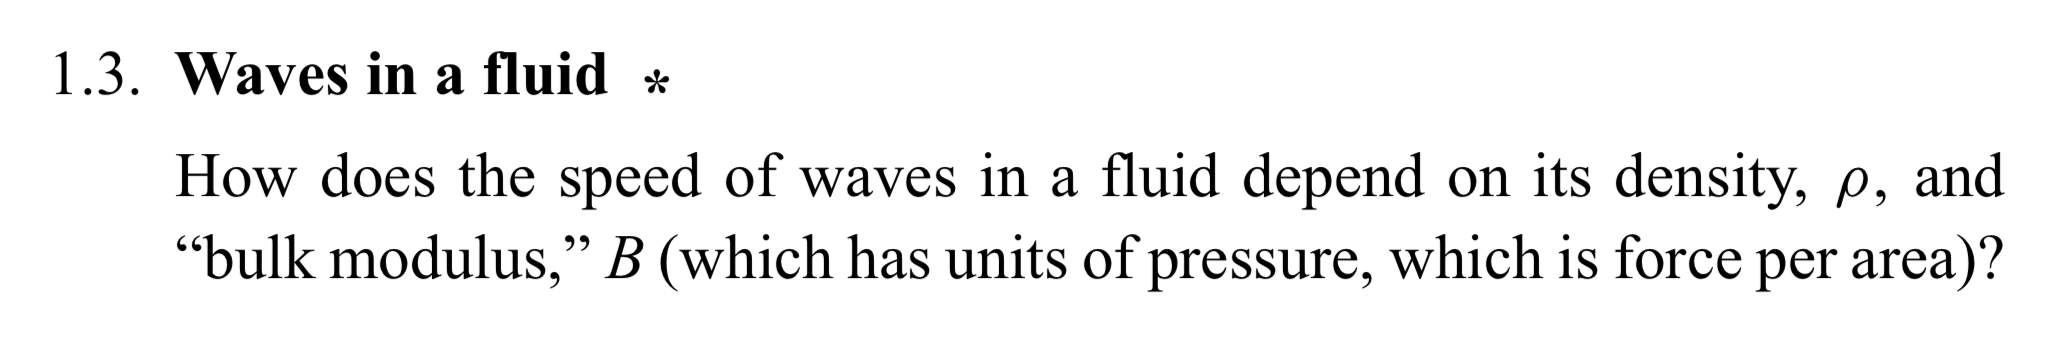
\includegraphics[width=400pt]{img/physics--classical-mechanics--morin--1-3.png}
\end{mdframed}

\begin{tabular}{l|l}
  speed   & $LT^{-1}$ \\
  density & $ML^{-3}$ \\
  bulk modulus & $MLT^{-2}L^{-2} = ML^{-1}T^{-2}$
\end{tabular}

\begin{align*}
  \matMMMxNN
  {-3}{-1}
  {1}{1}
  {0}{-2} \vecMM{i}{j} = \vecMMM{1}{0}{-1}.
\end{align*}
$\implies j = 1/2, i = -1/2$\\
So speed is proportional to $\sqrt{B/\rho}$. \checkmark

\subsubsection*{}
\begin{mdframed}
  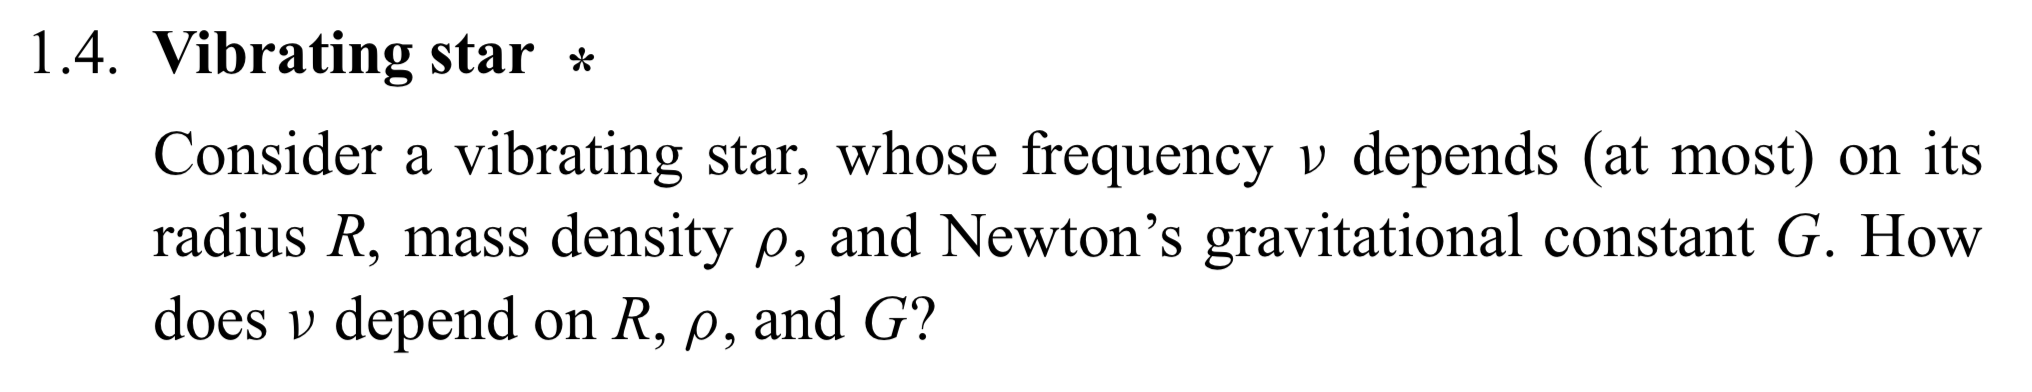
\includegraphics[width=400pt]{img/physics--classical-mechanics--morin--1-4.png}
\end{mdframed}
\begin{tabular}{l|l}
  Frequency $\nu$            & $T^{-1}$ \\
  Radius $R$                 & $L$ \\
  Mass density $\rho$        & $ML^{-3}$ \\
  Gravitational constant $G$ & $L^3M^{-1}T^{-2}$
\end{tabular}

Suppose $\nu \propto R^i\rho^jG^k$. Then $(i, j, k)^T$ would be a solution to
\begin{align*}
  \matMMMxNNN
  {1}{-3}{3}
  {0}{1}{-1}
  {0}{0}{-2} \vecMMM{i}{j}{k} = \vecMMM{0}{0}{-1}.
\end{align*}

$(0, 1/2, 1/2)$ is a solution, so frequency must be proportional to $\sqrt{G\rho}$. \checkmark

\subsubsection*{}
\begin{mdframed}
  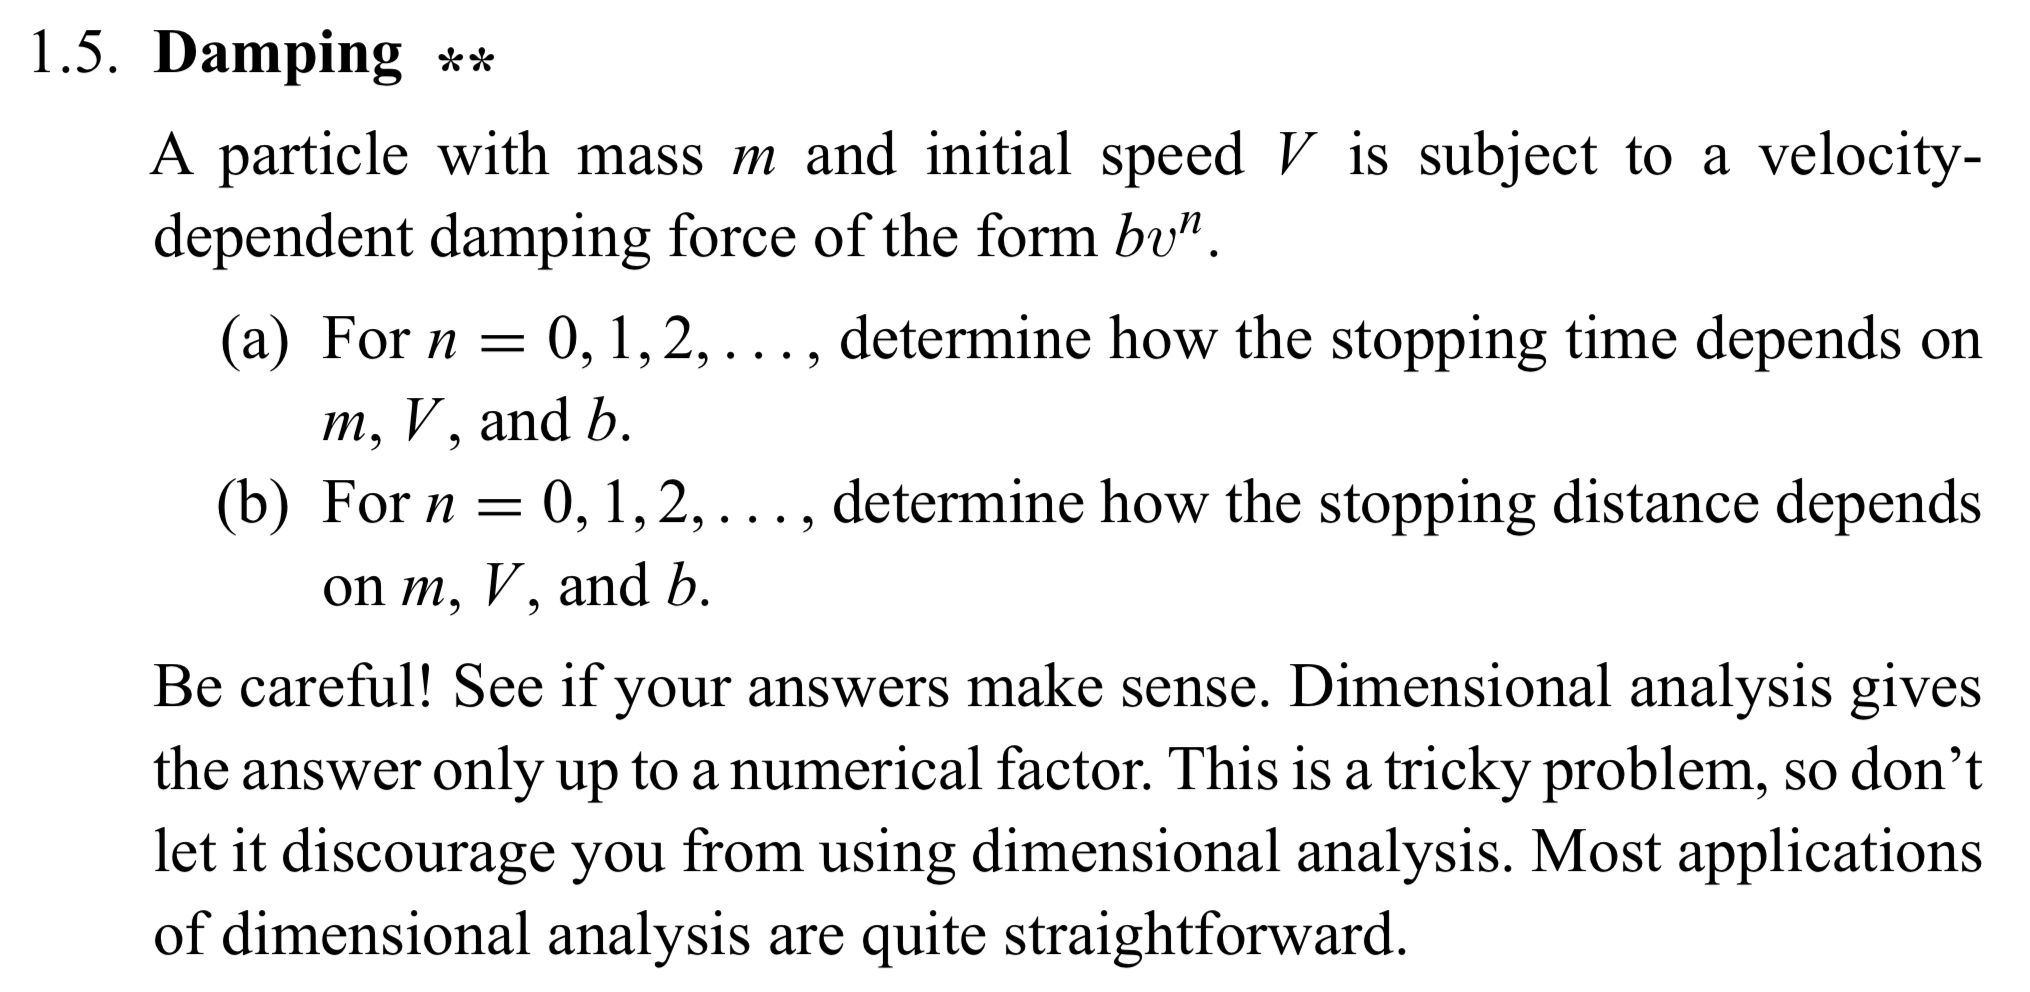
\includegraphics[width=400pt]{img/physics--classical-mechanics--morin--1-5.png}
\end{mdframed}

\begin{tabular}{l|l}
  Stopping time     & $T$ \\
  Stopping distance & $L$ \\
  \hline
  mass $m$          & $M$ \\
  Initial speed $V$ & $LT^{-1}$ \\
  Constant $b$      & $ML^{1-n}T^{n-2}$ \\
  \hline
  $v^n$             & $L^nT^{-n}$ \\
  Force $F = bv^n$  & $MLT^{-2}$
\end{tabular}

\begin{enumerate}[label=(\alph*)]
\item Stopping time\\
  Suppose $T \propto m^iV^jb^k$. Then
  \begin{align*}
    \matMMMxNNN
    {0}{1}{1-n}
    {1}{0}{1}
    {0}{-1}{n-2} \vecMMM{i}{j}{k} &= \vecMMM{0}{0}{1},
  \end{align*}
  so that
  \begin{align*}
    i + k &= 0 \\
    j + k(1 - n) &= 0 \\
    -j + k(n - 2) &= 1 \\
    k &= -1 \\
    i &= 1 \\
    j &= 1 - n.
  \end{align*}

\begin{verbatim}
#+begin_src mathematica :results pp
LinearSolve[{{0, 1, 1-n}, {1, 0, 1}, {0, -1, n-2}}, {0, 0, 1}]
#+end_src

#+RESULTS:
: {1, 1 - n, -1}
\end{verbatim}

  So we have
  \begin{align*}
    T \propto mV^{1 - n}/b.
  \end{align*}

  \begin{enumerate}
  \item $n = 0$\\
    $T \propto mV/b$. Makes sense.
  \item $n = 1$\\
    $T \propto m/b$. Why not dependent on $V$? Failure of dimensional analysis; dimensionless
    proportionality constant $f(n) = f(1) = \infty$.
  \item $n = 2$\\
    $T \propto m/(bV)$. Why decreasing with $V$? Again, $f(2) = \infty$.
  \end{enumerate}

\item Stopping distance\\
  Suppose $D \propto m^iV^jb^k$. Then
  \begin{align*}
    \matMMMxNNN
    {0}{1}{1-n}
    {1}{0}{1}
    {0}{-1}{n-2} \vecMMM{i}{j}{k} &= \vecMMM{1}{0}{0},
  \end{align*}
  so that
  \begin{align*}
    i + k &= 0 \\
    j + k(1 - n) &= 1 \\
    -j + k(n - 2) &= 0 \\
    k &= -1 \\
    i &= 1 \\
    j &= 2 - n.
  \end{align*}

\begin{verbatim}
#+begin_src mathematica :results pp
LinearSolve[{{0, 1, 1-n}, {1, 0, 1}, {0, -1, n-2}}, {1, 0, 0}]
#+end_src

#+RESULTS:
: {1, 2 - n, -1}
\end{verbatim}

  So we have
  \begin{align*}
    T \propto mV^{2 - n}/b.
  \end{align*}

  \begin{enumerate}
  \item $n = 0$\\
    $T \propto mV^2/b$. Makes sense.
  \item $n = 1$\\
    $T \propto mV/b$. Makes sense.
  \item $n = 2$\\
    $T \propto m/b$. Why not dependent on $V$?
  \end{enumerate}
\end{enumerate}

\subsection*{Approximations, limiting cases}

\subsubsection*{1.6}
\begin{mdframed}
  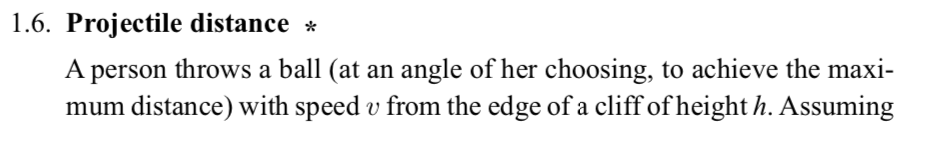
\includegraphics[width=400pt]{img/physics--classical-mechanics--morin--1-6-1.png}\\
  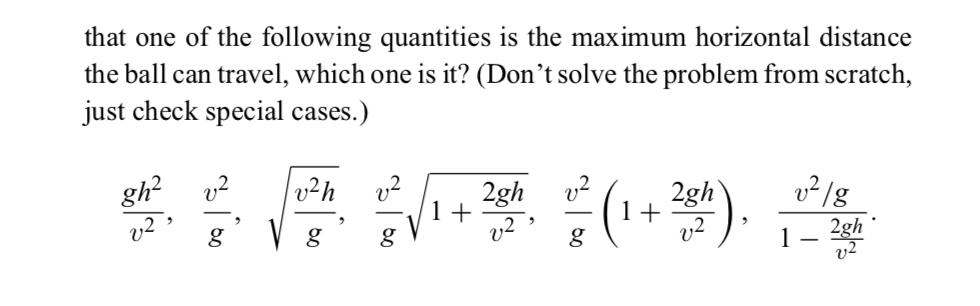
\includegraphics[width=400pt]{img/physics--classical-mechanics--morin--1-6-2.png}
\end{mdframed}

\begin{align*}
  [\frac{gh^2}{v^2}] &= \frac{L}{T^2} \frac{L^2}{1} \frac{T^2}{L^2} = L \checkmark \\
  [\frac{v^2}{g}]    &= \frac{L^2}{T^2} \frac{T^2}{L} = L \checkmark
\end{align*}

...

\subsubsection*{}
\begin{mdframed}
  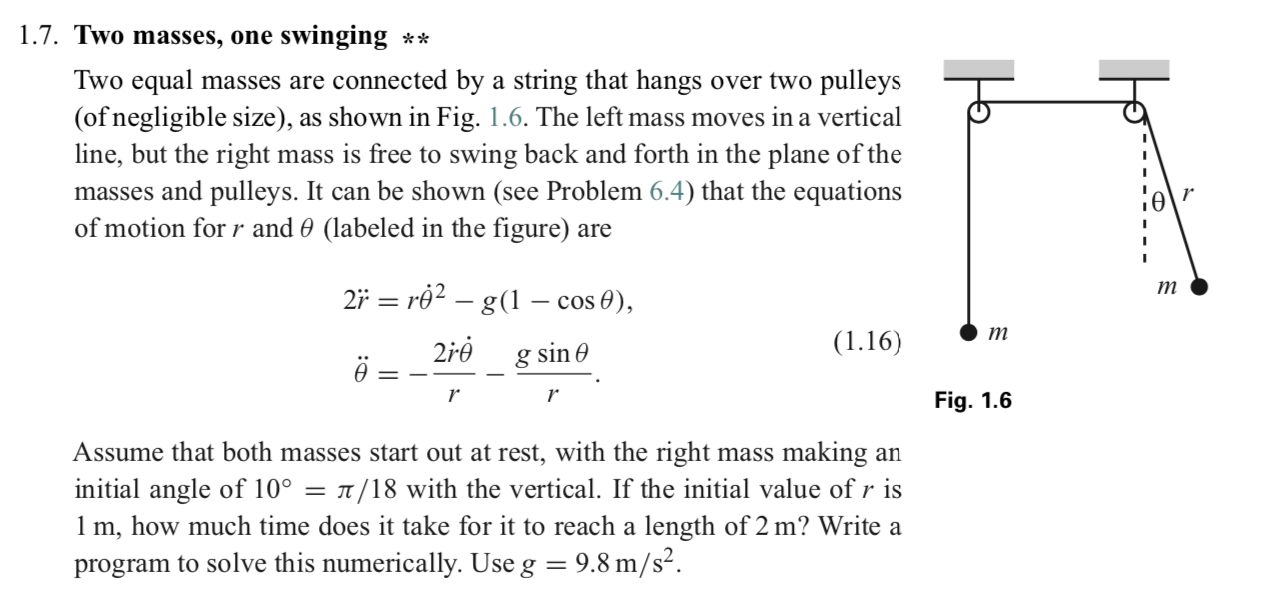
\includegraphics[width=400pt]{img/physics--classical-mechanics--morin--1-7.png}
\end{mdframed}

\begin{minted}{python3}
from dataclasses import dataclass
from math import cos
from math import pi
from math import sin

g = 9.8   # acceleration due to gravity (m/s)
dt = 0.0001  # tick interval (s)

@dataclass
class World:
    r: float = 1
    r_dot: float = 0
    theta: float = pi / 18
    theta_dot: float = 0
    time: float = 0

def r_dot_dot(self):
    return 0.5 * (self.r * self.theta_dot**2 - g*(1 - cos(self.theta)))

def theta_dot_dot(self):
    return -2 * self.r_dot * self.theta_dot / self.r - g * sin(self.theta) / self.r

def tick(self):
    self.r_dot += dt * self.r_dot_dot()
    self.r += dt * self.r_dot
    self.theta_dot += dt * self.theta_dot_dot()
    self.theta += dt * self.theta_dot
    self.time += dt


def main():
    world = World()
    while world.r < 2:
        world.tick()

    print(world.time)
\end{minted}

\section{Statics}
\subsection*{Balancing forces}
\subsubsection*{2.1}
\begin{mdframed}
  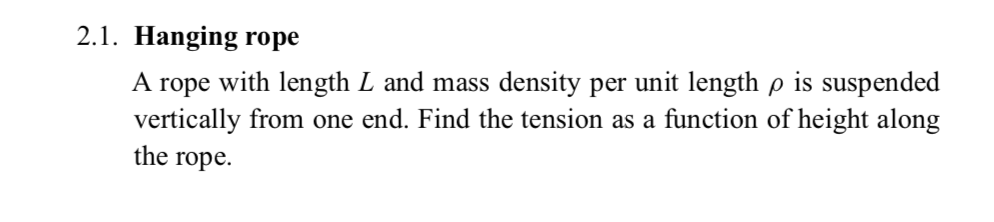
\includegraphics[width=400pt]{img/physics--classical-mechanics--morin--2-1.png}
\end{mdframed}

Let $h$ be height measured from the free (lower) end. The tension $F$ is due to the weight of the
section of the rope below:
\begin{align*}
  F = \rho hg,
\end{align*}
for $0 \leq h \leq L$. \checkmark

\begin{mdframed}
  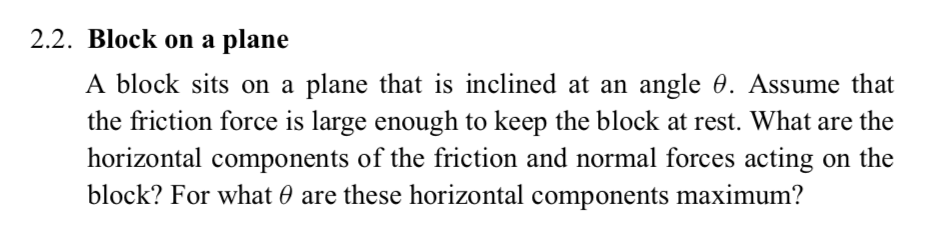
\includegraphics[width=400pt]{img/physics--classical-mechanics--morin--2-2.png}
\end{mdframed}

The normal force (component of weight normal to surface) is $mg\cos\theta$. The horizontal component
of this is $mg\cos\theta\sin\theta$.

Equivalently, the friction force (component of weight along surface) is $mg\sin\theta$. The
horizontal component of this is $mg\sin\theta\cos\theta$.

These are presumably maximum at $\theta = \pi/4$. \checkmark

\newpage
\subsubsection*{2.3}
\begin{mdframed}
  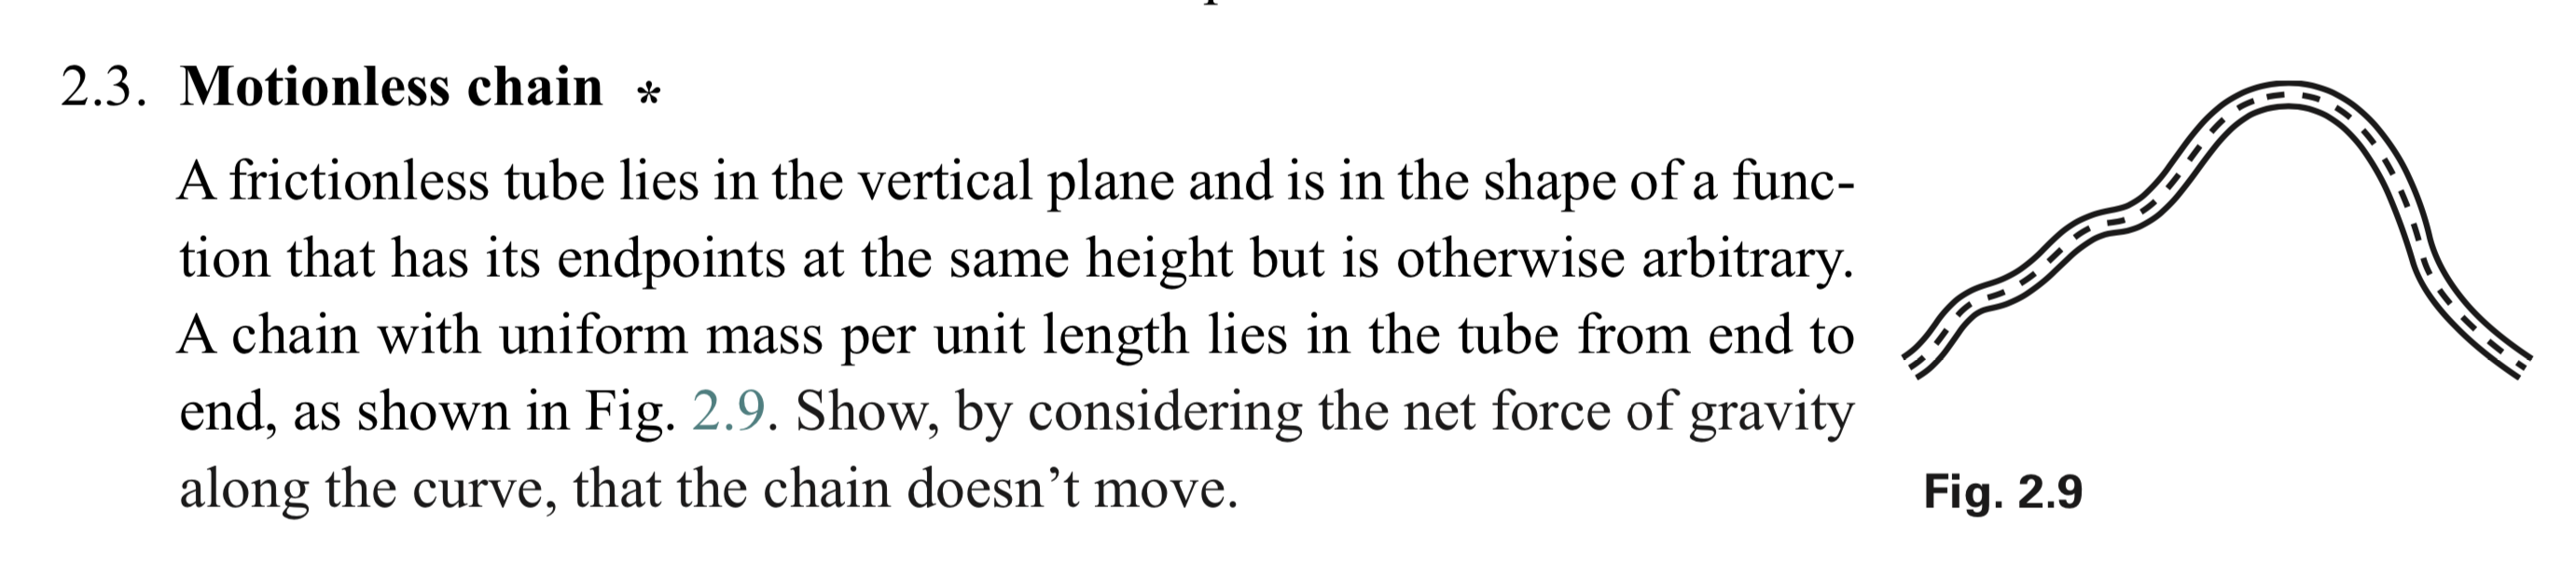
\includegraphics[width=400pt]{img/physics--classical-mechanics--morin--2-3.png}
\end{mdframed}

Focus on an arbitrary point $x$ along the horizontal axis. The height of the chain at this point is
$y(x)$ with tangent slope $\tan \theta = y'(x)$. Consider a short section of chain of length
$\dl = \sqrt{\dx^2 + \dy^2} = \sqrt{1 + \tan^2\theta} \dx$. Let the mass per unit length be
$\rho$. The weight is $\rho (\dl) g$ downwards. This has a component normal to the chain which we
can ignore, since it is balanced by the opposing normal force from the fixed tube. The component of
weight along the chain is $\rho (\dl) g \sin\theta$.

There will be tension and compression forces acting to oppose this component of weight, but we don't
need to analyse these. Instead we ask what the net force $F$ is \emph{along the chain}. Let $L$ be
the total length of the chain. We have

\begin{align*}
  F &= \int_{l=0}^{l=L} \rho g \sin\theta \dl \\
    &= \rho g \int_{l=0}^{l=L} \sin\theta \sqrt{1 + \tan^2\theta} \dx.
\end{align*}
Note that $\sin\theta = \frac{\tan\theta}{\sqrt{1 + \tan^2\theta}}$, and that $\tan\theta =
\dydx$. Therefore
\begin{align*}
  F &= \rho g \int_{l=0}^{l=L} \dy\\
    &= \rho g \(y(L) - y(0)\)\\
    &= 0.
\end{align*}

\newpage
\subsubsection*{2.4}
\begin{mdframed}
  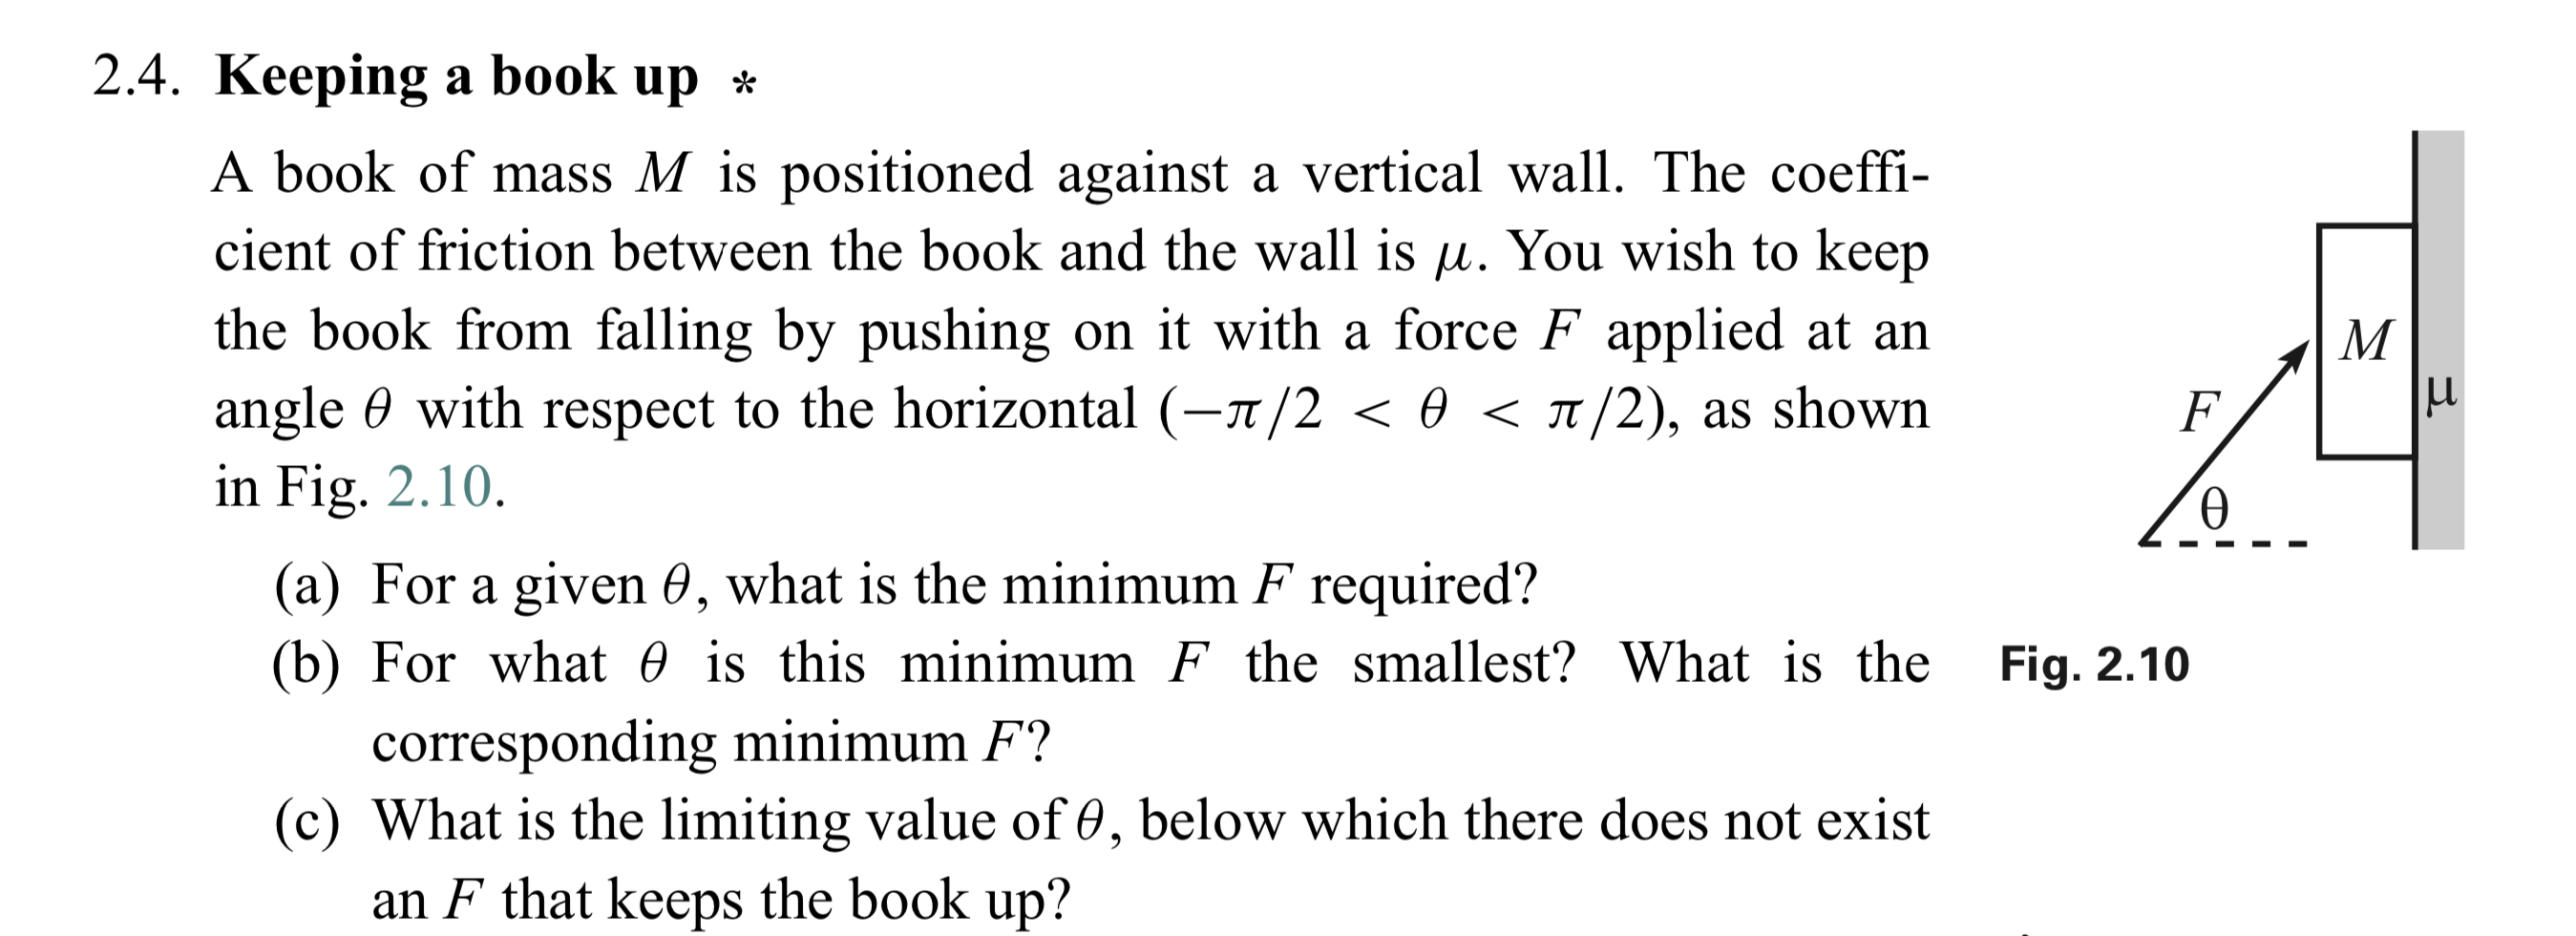
\includegraphics[width=400pt]{img/physics--classical-mechanics--morin--2-4.png}
\end{mdframed}

When $F = 0$, the book will fall down freely under the gravity force $Mg$.

The relevant forces are
\begin{itemize}
\item the book weight $Mg$,
\item an upwards supporting force of $S = F\sin\theta$ (which will be negative when $\theta < 0$,
  i.e. when $F$ is pointing downwards),
\item a normal force of $N = F\cos\theta$.
\end{itemize}

So, there is a downwards force of $D = W - S$. And therefore there is also an upwards friction force
of $\min\(\mu N, D\)$. When this is less than $D$, the book is sliding down.

Suppose $\theta$ is positive and $F$ is initially holding the book in place. This means that
$\mu N > D$. As $F$ decreases, it causes $S$ to decrease, which means that $D$ increases. At the
same time, $\mu N$ is decreasing. So $D$ and $\mu N$ are moving towards each other. When they meet,
the book is about to start sliding down.

\begin{enumerate}[label=(\alph*)]
\item The minimum $F$ occurs when $D = \mu N$. I.e.
  \begin{align*}
    W - S            &= \mu N \\
    Mg - F\sin\theta &= \mu F\cos\theta \\
    F &= \frac{Mg}{\sin\theta + \mu\cos\theta}.
  \end{align*}
  Makes sense: more force needed if book heavier; less force needed if $\mu$ larger ($\cos$ is
  positive in $(-\pi/2, \pi/2)$); \todo{change with $\theta$}.
\item We seek the $\theta \in (-\pi/2, \pi/2)$ which maximizes
  $g(\theta) = \sin\theta + \mu\cos\theta$. We have $g'(\theta) = \cos\theta - \mu\sin\theta$, and
  setting this equal to zero gives $\tan\theta = 1/\mu$. So, the minimum $F$ is smallest for
  $\theta = \tan^{-1}(1/\mu)$. This minimum $F$ is (using $\cos\theta = 1/\sqrt{1 + \tan^2\theta}$)
  \begin{align*}
    F
    &= \frac{Mg/\cos\theta}{\tan\theta + \mu} \\
    &= \frac{Mg\sqrt{1 + \tan^2\theta}}{\tan\theta + \mu} \\
    &= \frac{Mg\sqrt{1 + 1/\mu^2}}{1/\mu + \mu}.
  \end{align*}

  \todo{Book gives $\frac{Mg}{\sqrt{1 + \mu^2}}$}

\begin{verbatim}
#+begin_src mathematica :results raw pp
Simplify[Sqrt[1 + 1/mu^2]/(1/mu + mu)]
#+end_src

#+RESULTS:
: (Sqrt[1 + mu^(-2)]*mu)/(1 + mu^2)

\end{verbatim}

\item As $\theta$ decreases below zero, $D$ increases ($S$ is now negative) and $\mu N$
  decreases. The limiting...\todo{}
\end{enumerate}

\subsubsection*{2.9}
Recall from \ref{foundations-hyperbolic-trig-functions} that
\begin{align*}
  \cosh x &= \frac{e^x + e^{-x}}{2} \\
  \sinh x &= \frac{e^x - e^{-x}}{2},
\end{align*}
therefore
\begin{align*}
  \ddx \cosh x &= \sinh x \\
  \ddx \sinh x &= \cosh x,
\end{align*}
and
\begin{align*}
  \cosh^2 x             &= \frac{1}{4}\(e^{2x} + e^{-2x}\) + \frac{1}{2} \\
  \sinh^2 x             &= \frac{1}{4}\(e^{2x} + e^{-2x}\) - \frac{1}{2} \\
  1 + \sinh^2 x         &= \cosh^2 x \\
  \sinh^2 x + \cosh^2 x &= \cosh 2x.
\end{align*}

\begin{mdframed}
  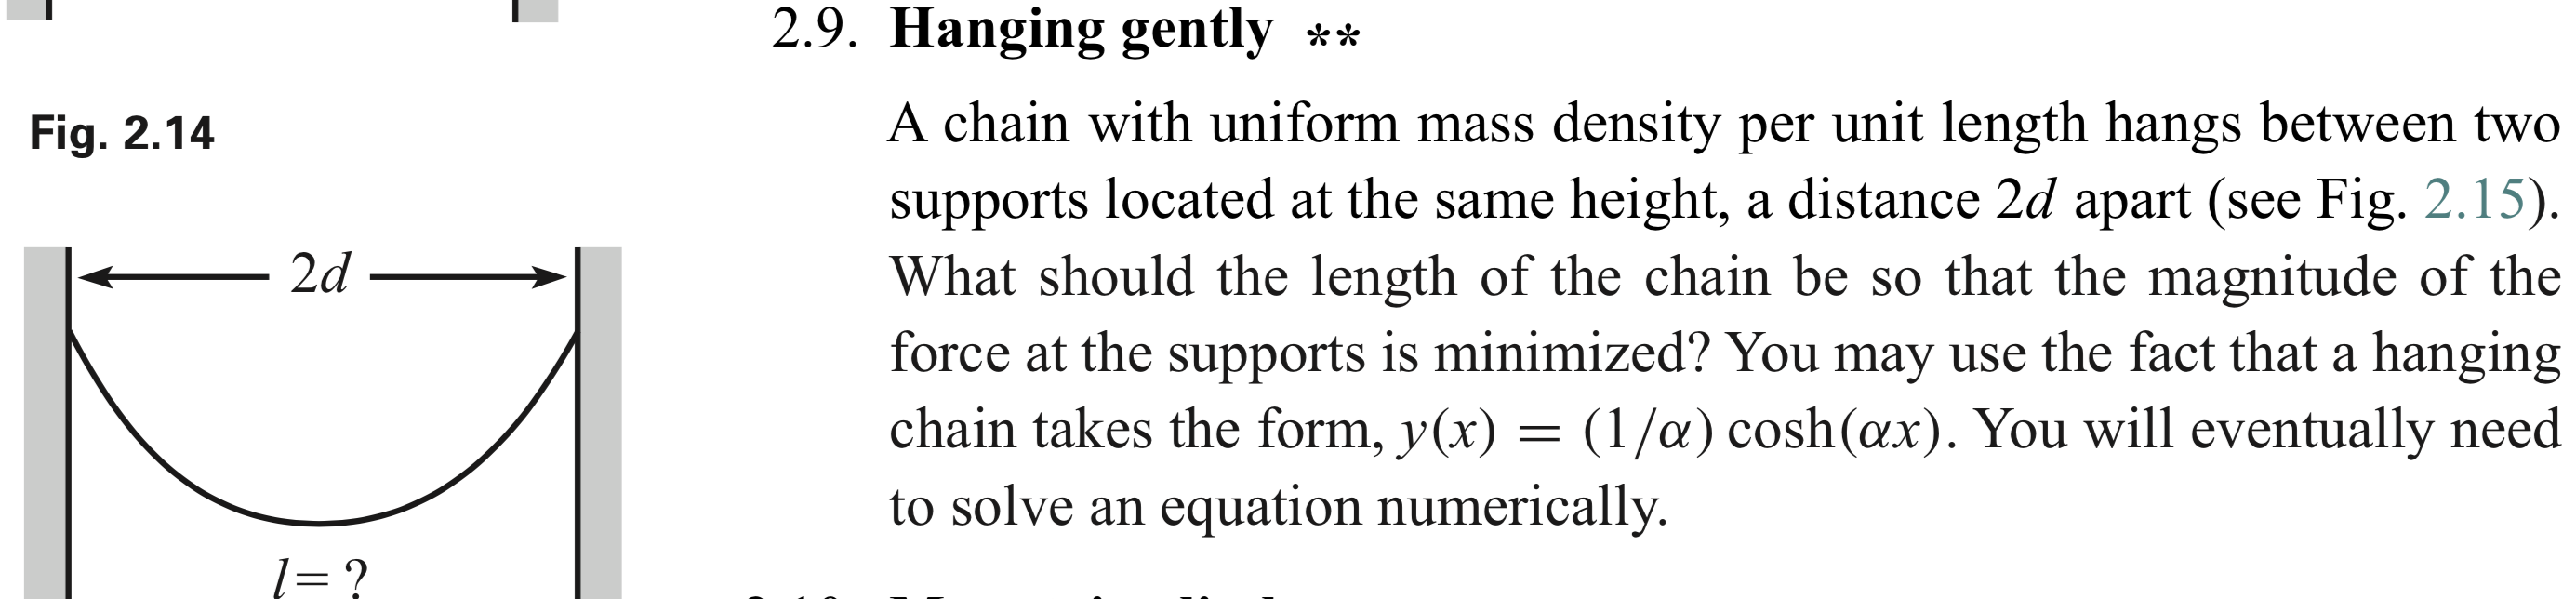
\includegraphics[width=400pt]{img/physics--classical-mechanics--morin--2-9.png}
\end{mdframed}

Let $x = 0$ be the centre point of the chain, so that the left end is at $-d$ and the right end at
$d$.

The height of the chain at $x$ is $y(x) = (1/\alpha)\cosh \alpha x$ and the slope of the chain at
$x$ is $y'(x) = \sinh \alpha x$.

Let the length of the chain be $l$ with density $\rho$.

We can calculate $l$, since we know the form of the curve: consider a short horizontal region of
length $\Delta x$. Making a linear approximation to the curve, the length is given by
\begin{align*}
  (\Delta l)^2            &= (\Delta x)^2 + (y'(x)\Delta x)^2 \\
                          &= \(1 + y'(x)^2\)(\Delta x)^2\\
  l = \int_{x=-d}^{x=d}\dl  &= \int_{x=-d}^{x=d} \sqrt{1 + y'(x)^2} \dx \\
                          &= \int_{x=-d}^{x=d} \sqrt{1 + \sinh^2 \alpha x} \dx \\
                          &= \int_{x=-d}^{x=d} \cosh \alpha x \dx \\
                          &= \frac{1}{\alpha}\(\sinh (\alpha d) - \sinh (-\alpha d)\) \\
                          &= 2\frac{\sinh(\alpha d)}{\alpha}. ~~~~~~~\checkmark
\end{align*}

The total weight of the chain is $\rho l g$, and since the system is left-right symmetric, each of
the supports bears half the weight of the chain. Therefore at the right attachment point we have a
force diagram with hypotenuse $F$ (the force on the chain at the attachment point, acting along the
chain, upwards and to the right at an angle $\theta$ to the horizontal), and vertical upwards
component equal to half the weight of the chain. So, we have
\begin{align*}
  F\sin\theta = (\rho g)\frac{\sinh(\alpha d)}{\alpha}.
\end{align*}

Note however that $\alpha$ and $\theta$ are not independent parameters: one determines the other. We
want an expression with a single parameter that we can then minimize to find the parameter value
that results in the minimum force $F$.

The dependence of $\theta$ and $\alpha$ is given by the expression for the slope of the curve at the
attachment point:
\begin{align*}
  \tan\theta = \sinh(\alpha d),
\end{align*}
and this allows us to write $\sin\theta$ as a function of $\alpha$ as follows: it means that at the
right end, for every one unit moved horizontally, the chain rises by $\sinh(\alpha d)$. Using the
identity $1 + \sinh^2\phi = \cosh^2\phi$, this implies that the hypotenuse of such a triangle is
$\cosh(\alpha d)$, and therefore that
$\sin\theta = \frac{\sinh(\alpha d)}{\cosh(\alpha d)} = \tanh(\alpha d)$.

\begin{mdframed}
  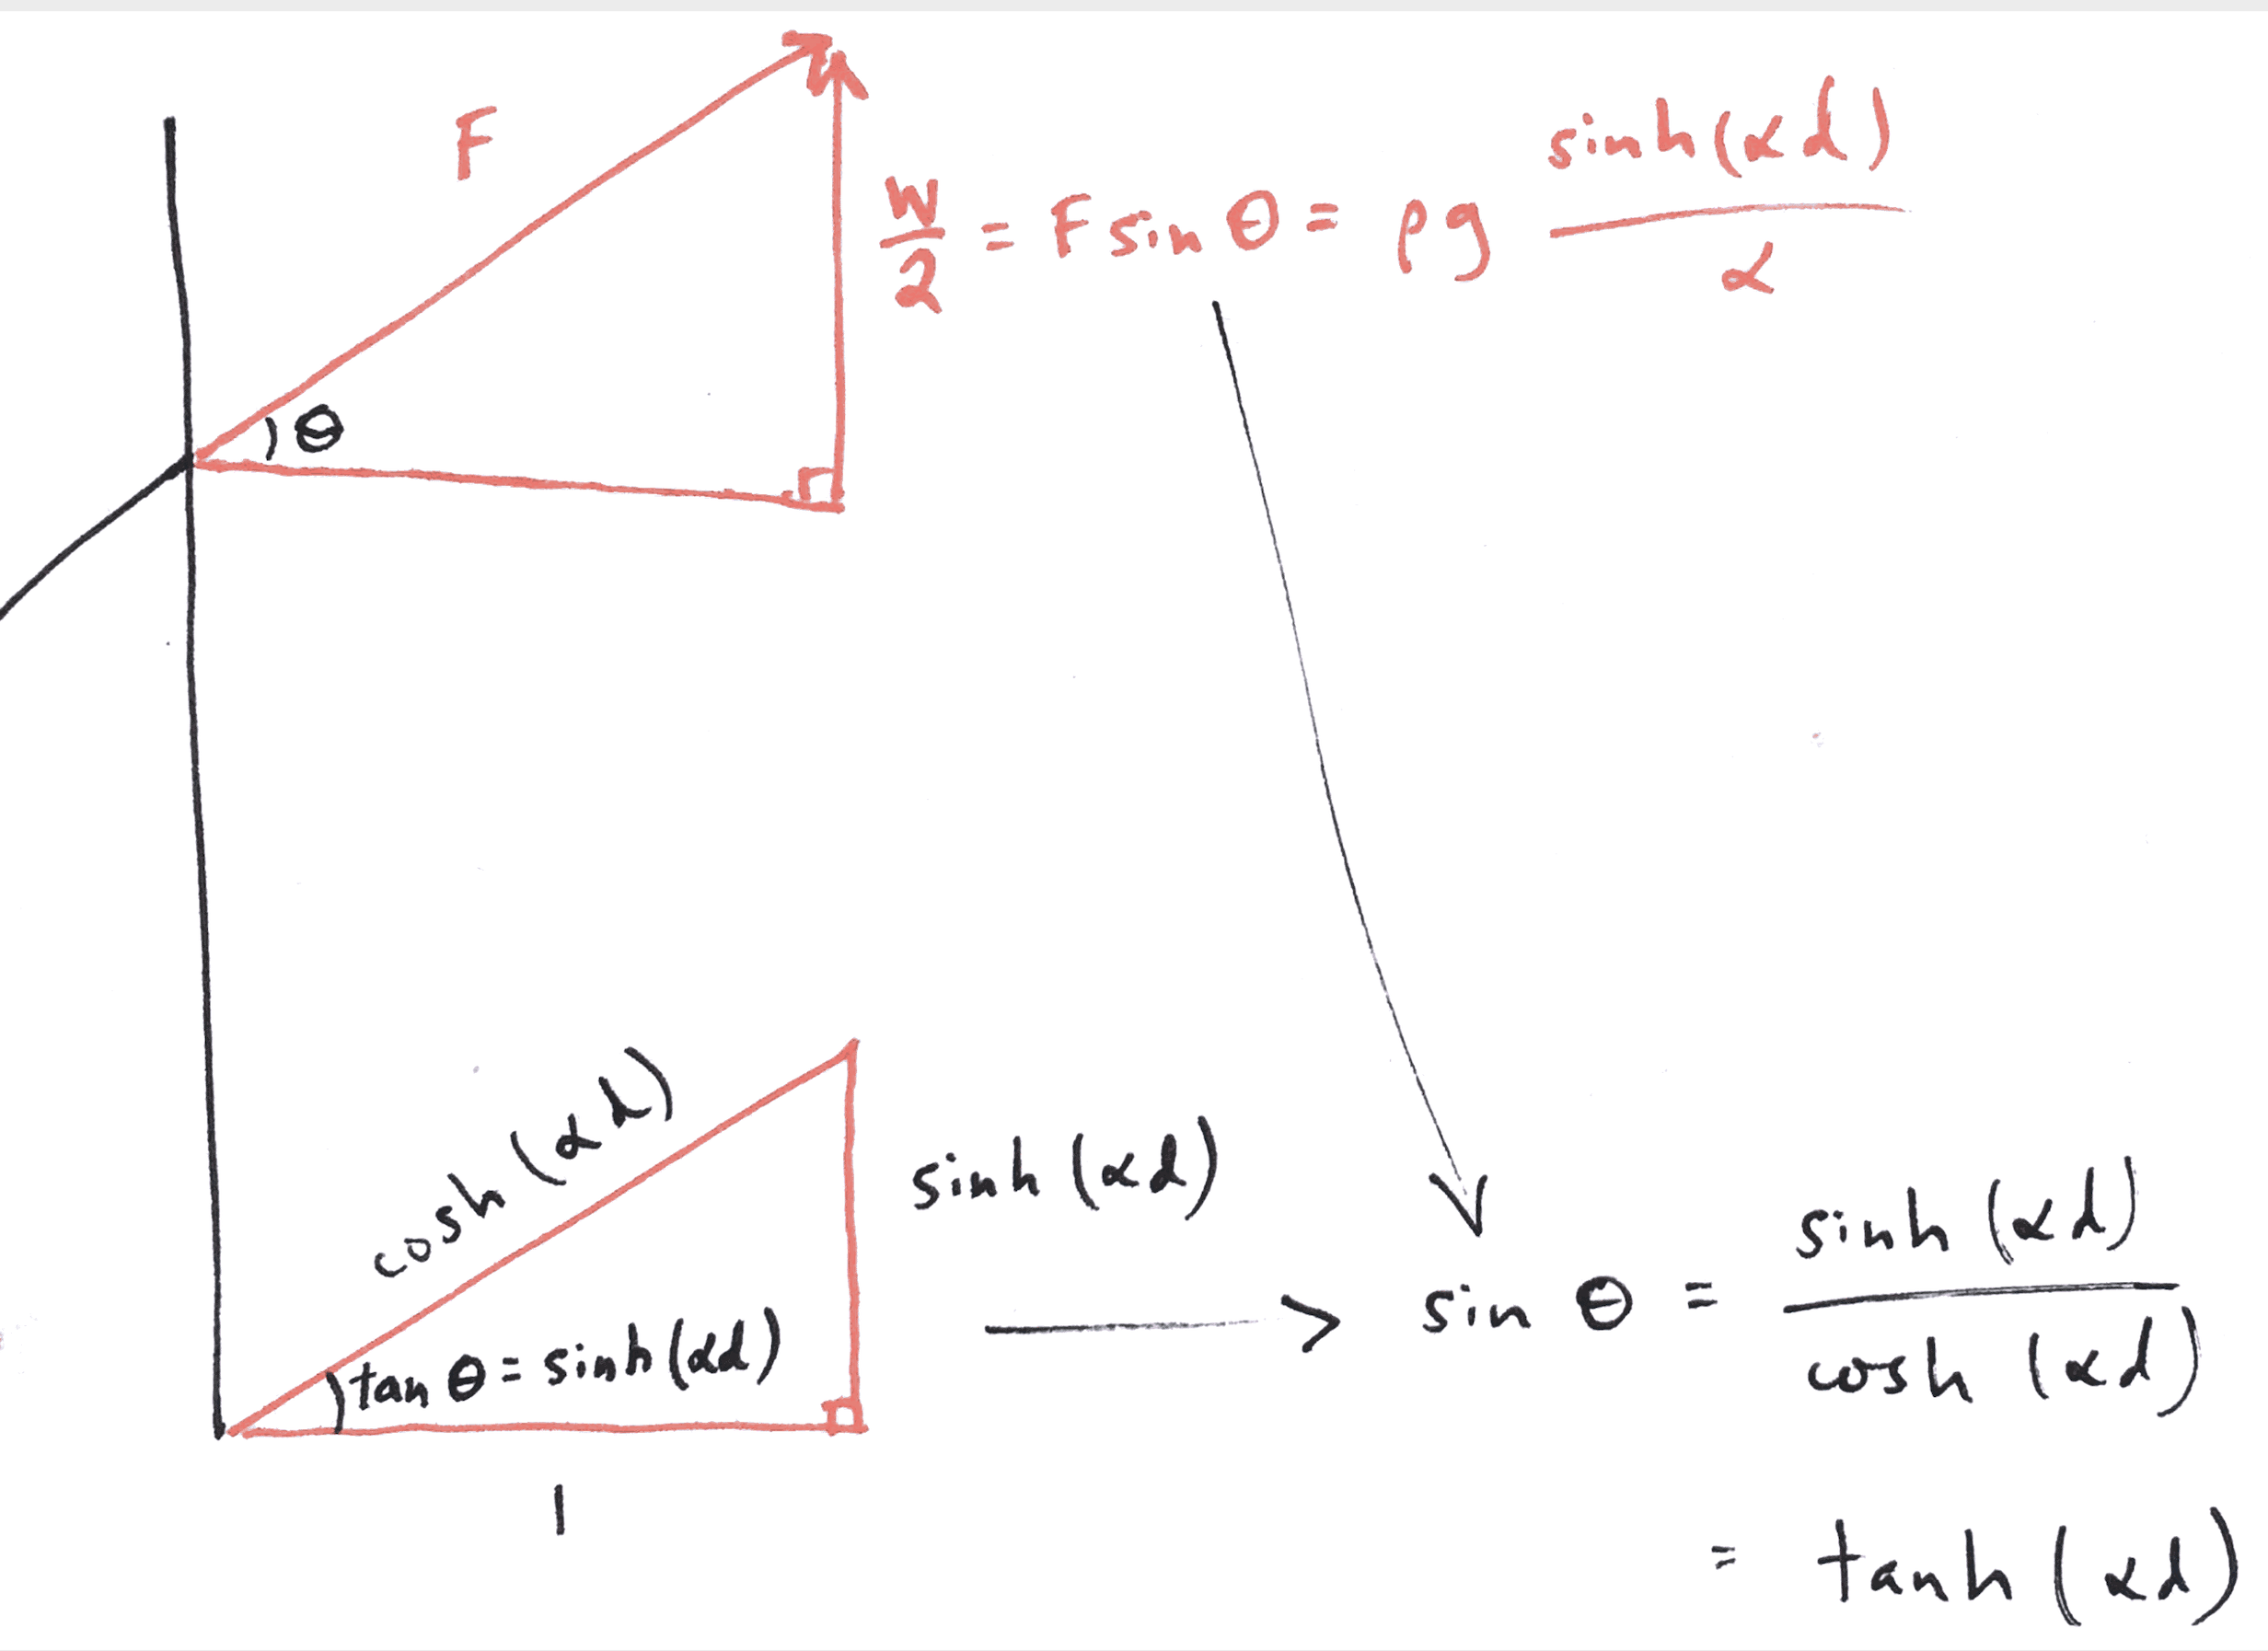
\includegraphics[width=300pt]{img/physics--classical-mechanics--morin--2-9-diagram.png}
\end{mdframed}

Thus we have an expression for $F$ in terms of the single parameter $\alpha$:
\begin{align*}
  F = (\rho g)\frac{\sinh(\alpha d)}{\alpha \tanh(\alpha d)} = (\rho g)\frac{\cosh(\alpha d)}{\alpha}, ~~~~~~~\checkmark
\end{align*}
and all that remains is to minimize this over $\alpha$:
\begin{align*}
  (1/\rho g)\frac{\dif}{\dif\alpha} F &= d\sinh(\alpha d)\alpha^{-1} -\alpha^{-2}\cosh(\alpha d) \\
                                      &= \frac{\alpha d \sinh(\alpha d) - \cosh(\alpha d)}{\alpha^2} \\
                                      &= 0 \\
                      \tanh(\alpha d) &= \frac{1}{\alpha d}. ~~~~~~~\checkmark
\end{align*}

\begin{verbatim}
#+begin_src mathematica :results pp
NSolve[Tanh[ad] == 1/(ad), ad, Reals]
#+end_src

#+RESULTS:
: {{ad -> -1.1996786402577337}, {ad -> 1.1996786402577337}}
\end{verbatim}


\todo{Consider a short section of chain. It has weight acting vertically downwards, which can be
  resolved into a component along the chain and a component normal to the chain. The component along
  the chain is balanced by equal and opposite tension (and compression?) forces within the
  chain. But what is the component of the weight normal to the chain balanced by?}

\newpage

\subsection*{Balancing torques}

\subsection*{Example: Leaning ladder}
\begin{mdframed}
  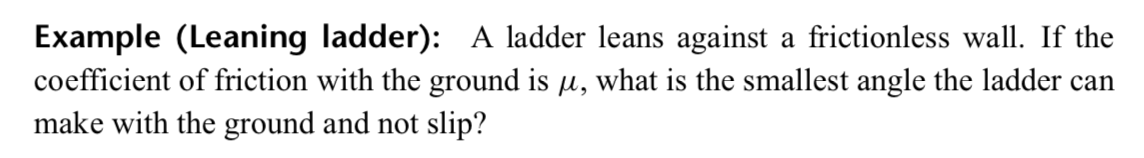
\includegraphics[width=400pt]{img/physics--classical-mechanics--morin--2--torque-example.png}\\
  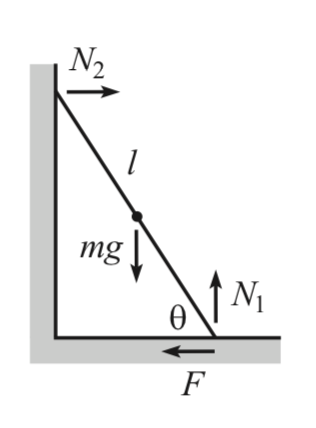
\includegraphics[width=100pt]{img/physics--classical-mechanics--morin--2--torque-example-diag.png}
\end{mdframed}

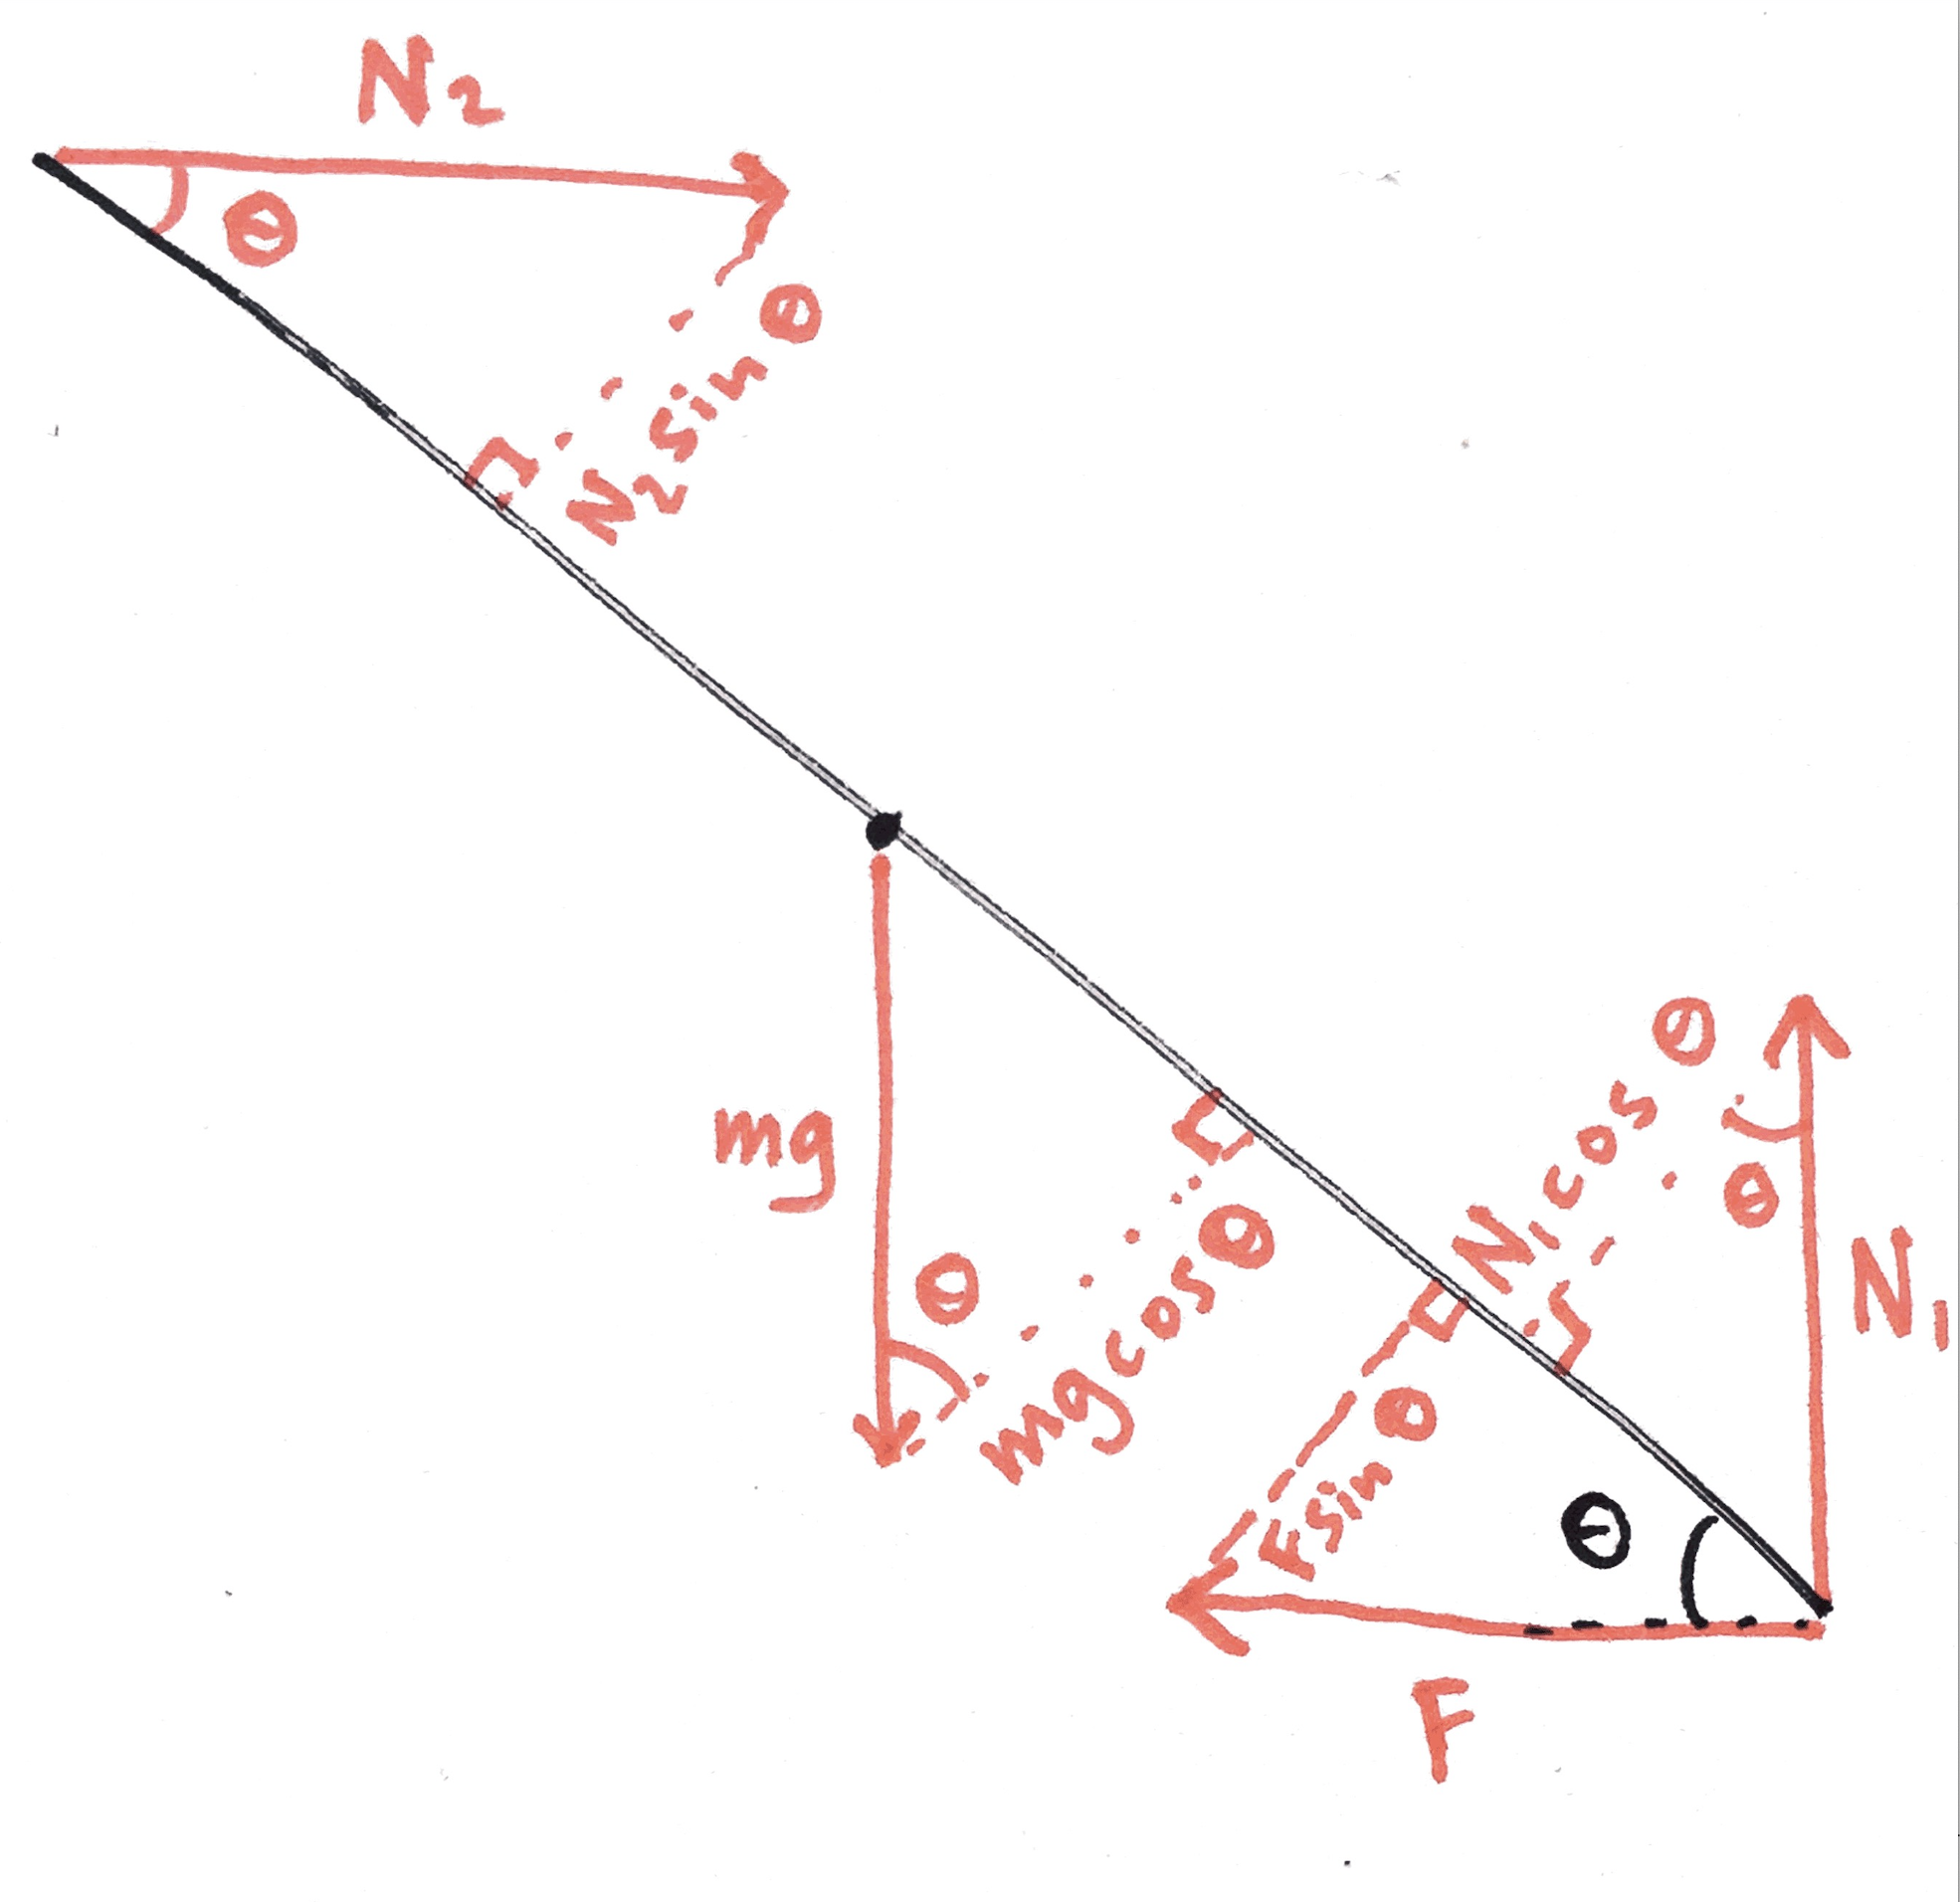
\includegraphics[width=150pt]{img/physics--classical-mechanics--morin--2--torque-example-diag-2.png}

We can make the following statements about the system:
\begin{enumerate}
\item There is a vertical weight force acting downwards and it is balanced by a vertical reaction
  from the ground: $N_1 = -mg$ (since the wall is frictionless, there is no vertical force there).
\item There are also some horizontal forces. Basically, although the weight has no horizontal
  component, it \emph{does} have a component normal to the ladder. This is $mg\cos\theta$,
  effectively acting at a distance $l/2$ from the toe of the ladder. If we were to remove the wall,
  the ladder would rotate around its toe due to this torque. So the wall must be doing something to
  balance this rotation. What it's doing is exerting a horizontal normal/reaction force $N_2$. The
  component of this normal to the ladder is $N_2\sin\theta$, acting at a distance $l$ from the
  toe. These torques around the toe must balance, hence
  \begin{align*}
    (l/2)mg\cos\theta &= lN_2\sin\theta \\
    N_2               &= \frac{mg}{2\tan\theta}.
  \end{align*}
\item The horizontal normal force $N_2$ at the wall (required to balance the torque induced by the
  weight), is opposed by a friction force: $F = -N_2$.
\item So for given $\theta$, we have determined $N_1$, $N_2$, and $F$. However, we could also
  analyze torques around the contact point with the wall:
  \begin{align*}
    (l/2)mg\cos\theta + lF\sin\theta &= lN_1\cos\theta \\
    N_1                              &= mg/2  + F\tan\theta.
  \end{align*}
  This should be consistent with the above solutions. Let's check that: the LHS is $N_1 = -mg$. And
  the RHS is
  \begin{align*}
  mg/2 + F\tan\theta = mg/2 + \frac{-mg}{2\tan\theta}\tan\theta = 0 ~~~~~~~\red{!}
  \end{align*}
  \todo{So it looks like there's some sign confusion.}
\end{enumerate}


So to answer the question, the smallest angle the ladder can make with the ground without slipping
is $\theta$ such that
\begin{align*}
  F = \frac{mg}{2\tan\theta} &= \mu N_1 = \mu m g \\
  \tan\theta                 &= 1/(2\mu).
\end{align*}
Sanity check: a larger coefficient of friction permits a shallower angle.


\newpage
\subsection*{2.11}
\begin{mdframed}
  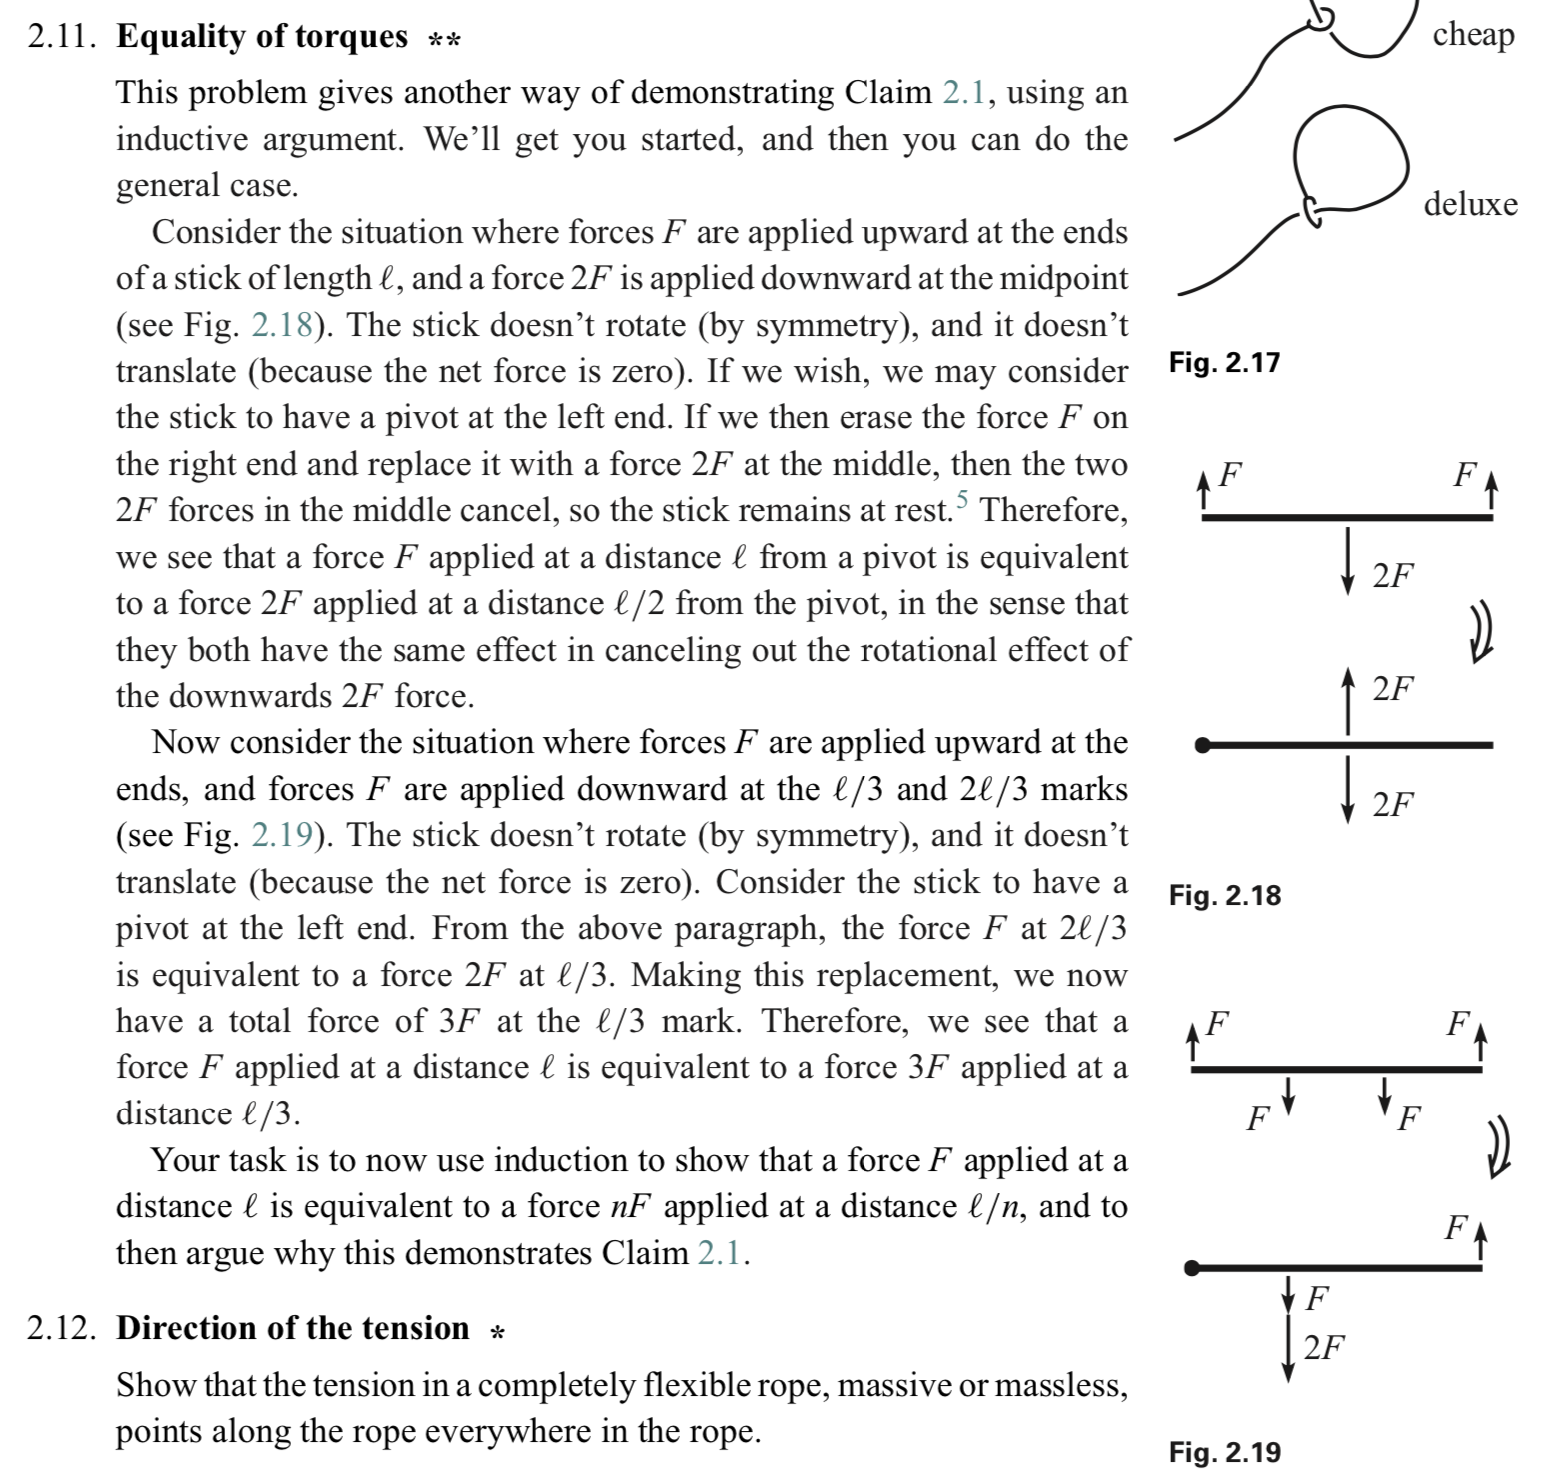
\includegraphics[width=400pt]{img/physics--classical-mechanics--morin--2-11.png}
\end{mdframed}
\newpage
\section{Using $F = ma$}
\subsection*{Free-body diagrams}

\subsubsection*{3.1 Atwood's machine}
\begin{mdframed}
  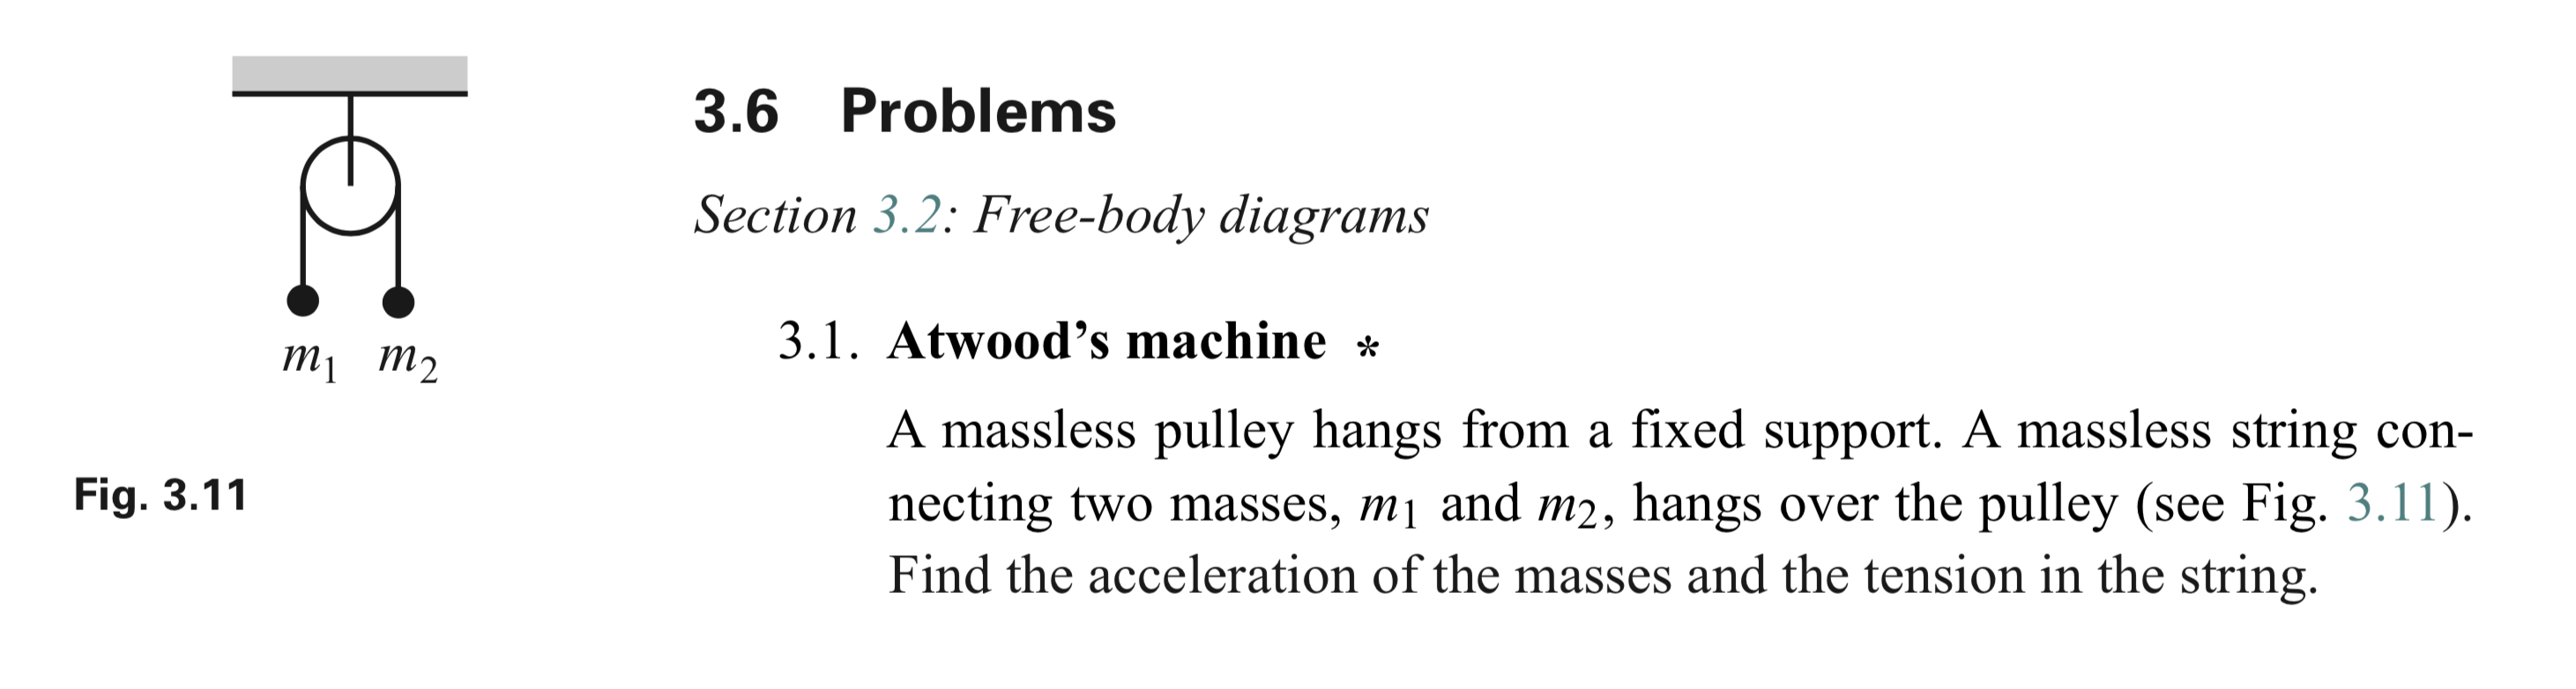
\includegraphics[width=400pt]{img/physics--classical-mechanics--morin--3-1.png}
\end{mdframed}
Let $a$ be the rightward acceleration of the string, and $T$ be the tension in the string.

To find $a$ is simple: there is a net force of $F = m_2g - m_1g$, therefore
\begin{align}
  a = \frac{F}{m} = \frac{m_2g - m_1g}{m_1 + m_2}. \label{morin-3-1-a} ~~~~~~~\checkmark
\end{align}
However, this doesn't give $T$.

Below are two ways to find $T$ by using $F = ma$ at each mass:
\begin{enumerate}
\item by substituting the above expression for $a$ into either one of them,
\item by solving the two jointly as a linear system, without using the above expression for $a$.
\end{enumerate}

So it seems that the acceleration of the whole system can be found using ``one degree of
freedom''(?), but that finding the tension requires solving a two-dimensional linear system.

Using $F = ma$ at each mass, we have
\begin{align}
  m_1a &= T-m_1g   \label{morin-3-1-Fma1}\\
  m_2a &= m_2g - T \label{morin-3-1-Fma2}.
\end{align}
From \eqref{morin-3-1-a} and \eqref{morin-3-1-Fma1} we have
\begin{align*}
  T &= \frac{m_1(m_2g - m_1g)}{m_1 + m_2} + m_1g \\
    &= \frac{2m_1m_2g}{m_1 + m_2}. ~~~~~~~\checkmark
\end{align*}
And as a check, from \eqref{morin-3-1-a} and \eqref{morin-3-1-Fma2} we have
\begin{align*}
  T &= m_2g - \frac{m_2(m_2g - m_1g)}{m_1 + m_2} \\
    &= \frac{2m_1m_2g}{m_1 + m_2}.
\end{align*}

Alternatively, we can solve the linear system given by $F = ma$ at each mass:
\begin{align*}
  m_1a - T &= -m_1g \\
  m_2a + T &= m_2g,
\end{align*}
which can be solved by inverting the $2 \times 2$ matrix:
\begin{align*}
  \mat{m_1}{-1}
      {m_2}{1} \vecMM{a}{T} &= \vecMM{-m_1g}{m_2g} \\
  \vecMM{a}{T}              &= \frac{1}{m_1 + m_2} \mat{1}{1}
                                                       {-m_2}{m_1} \vecMM{-m_1g}{m_2g} \\
                            &= \frac{1}{m_1 + m_2} \vecMM{m_2g - m_1g}{2m_1m_2}. ~~~~~~~\checkmark
\end{align*}

\subsubsection*{3.2 Double Atwood's machine}
\begin{mdframed}
  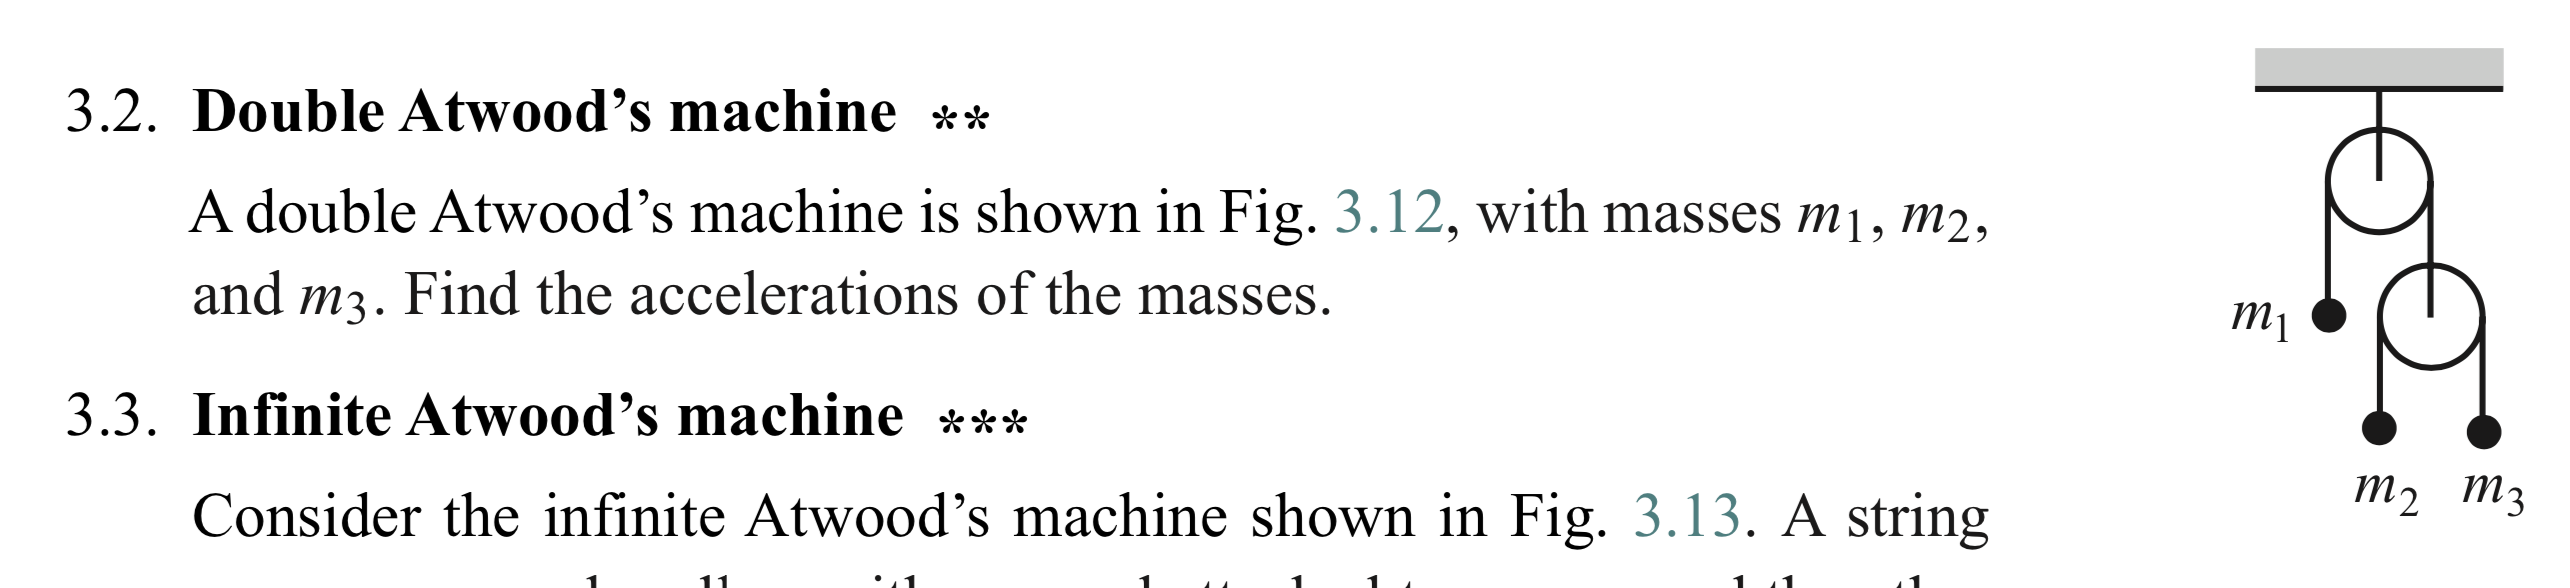
\includegraphics[width=400pt]{img/physics--classical-mechanics--morin--3-2.png}
\end{mdframed}
Define upward acceleration to be positive. So for example the net force acting on mass $m_1$ is
$T_1 - G\frac{Mm_1}{R^2}$, where $M$ and $R$ are the mass and radius of Earth. We usually denote
$G\frac{M}{R^2}$ as $g = 9.8ms^{-2}$, so we have
\begin{align*}
  m_1a_1 &= T_1 - m_1g \\
  a_3 &= -a_2 \\
  ...
\end{align*}



\subsection*{Solving differential equations}
\subsubsection*{}
\begin{mdframed}
  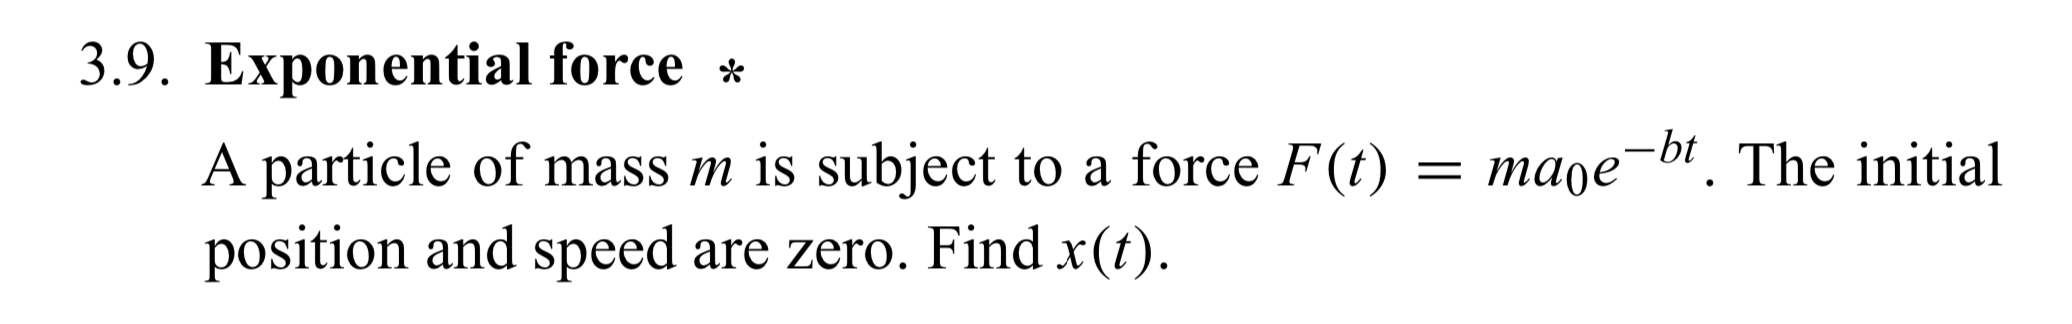
\includegraphics[width=400pt]{img/physics--classical-mechanics--morin--3-9.png}
\end{mdframed}

The position $x$ evolves according to the following differential equation:
\begin{align*}
  m\ddot{x} = F(t) = ma_0e^{-bt}.
\end{align*}
Thus \todo{Don't think these are correct; confused about exponentials}:
\begin{itemize}
\item The sign of $a_0$ determines the direction of motion.
\item If $b < 0$ then the particle is subject to exponentially increasing acceleration and thus
  super-exponentially increasing velocity without limit.
\item If $b = 0$ then the particle is subject to constant force, i.e. constant acceleration,
  i.e. velocity increases exponentially.
\item If $b > 0$ then the particle is subject to exponentially decreasing acceleration. It will
  start with close-to exponentially increasing velocity and approach a constant limiting velocity
  from below.
\end{itemize}

Note that if $m = 0$ then there is no force and the particle does not move; otherwise, we can divide
by $m$, removing dependence of the differential equation on $m$. We can then find $x(t)$ by
integrating twice:
\begin{align*}
  \frac{\d v}{\dt}                               &= a_0e^{-bt} \\
  \int_{v(0) = 0}^{v(t)} \d v = v(t) = \frac{\dx}{\dt} &= a_0 \int_0^t e^{-bt'} \dt'
                                                 = a_0 \(\frac{-1}{b}e^{-bt} + \frac{1}{b}\) \\
  \int_{x(0) = 0}^{x(t)}\dx = x(t)                    &= a_0 \int_0^{t}\(\frac{-1}{b}e^{-bt'} + \frac{1}{b}\) \dt'
                                                 = a_0\(\frac{1}{b^2}e^{-bt} + \frac{t}{b} - \frac{1}{b^2}\). \checkmark
\end{align*}

\todo{That doesn't handle $b = 0$}.

\begin{verbatim}
#+begin_src mathematica :results pp
Integrate[Integrate[m a0 Exp[-b __t], {__t, 0, _t}], {_t, 0, t}]
#+end_src

#+RESULTS:
: Integrate[Integrate[(a0*m)/E^(b*__t), {__t, 0, _t}], {_t, 0, t}]

\end{verbatim}



\subsubsection*{3.10}
\begin{mdframed}
  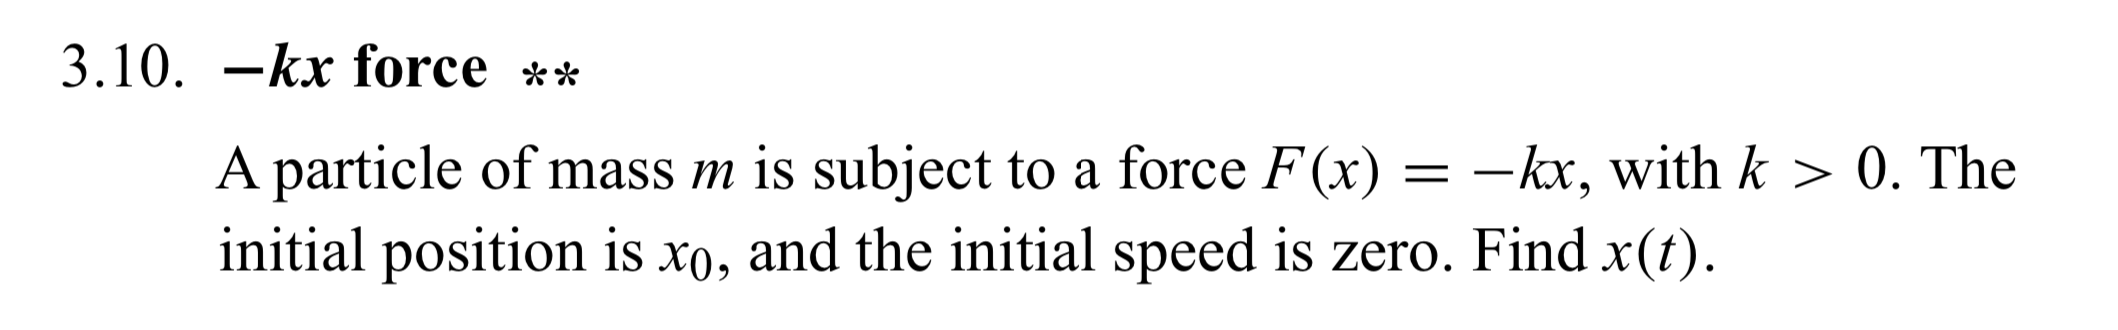
\includegraphics[width=400pt]{img/physics--classical-mechanics--morin--3-10.png}
\end{mdframed}

We want to find $x(t)$. We are given
\begin{align*}
  \ddot{x}  &= -\frac{k}{m}x \\
  \dot{x}(0) &= 0 \\
  x(0)       &= x_0,
\end{align*}
where $k > 0$.

Suppose $x(t) = Ae^{at}$. Then
\begin{align*}
  \dot{x}  &= Aae^{at} = ax \\
  \ddot{x} &= Aa^2e^{at} = a^2x.
\end{align*}

Therefore $x(t) = Ae^{at}$ is a solution iff $a^2 = -k/m$. So the solutions are linear combinations
of the form
\begin{align*}
  x(t) = Ae^{i\omega t} + Be^{-i\omega t},
\end{align*}
where $\omega = \sqrt{k/m} > 0$.

\red{Alternatively, this can be written as
\begin{align*}
  x(t) &= A(\cos\omega t + i\sin \omega t) + B(\cos\omega t - i\sin\omega t) \\
       &= (A + B)\cos\omega t + (A - B)i\sin \omega t,
\end{align*}
which shows that we must have $A = B$ in order that $x(t)$ is real-valued. Then $x(0) = x_0$
implies that $A + B = x_0$, giving the solution $x(t) = x_0\cos\omega t$. So the requirement for
real-valued solution means we don't need the initial velocity?}

The derivatives of such a solution are
\begin{align*}
    \dot{x} &= Ai\omega e^{i\omega t} - Bi\omega e^{-i\omega t}
             = i\omega\(A e^{i\omega t} - B e^{-i\omega t}\) \\
  \ddot{x}  &= -A\omega^2 e^{i\omega t} - B\omega^2 e^{-i\omega t} = -\omega^2x(t).
\end{align*}
(The expression for $\ddot{x}$ confirming that any such linear combination is a solution.)

The initial velocity condition $\dot{x}(0) = 0$ yields $A = B$, and hence the initial position
condition $x(0) = x_0$ yields $A = \frac{x_0}{2}$. Hence the solution is
\begin{align*}
  x(t) &= \frac{x_0}{2}\(e^{i\omega t} + e^{-i\omega t}\) \\
       &= \frac{x_0}{2}(2\cos\omega t) \\
       &= x_0\cos\(\sqrt{\frac{k}{m}} t\).
\end{align*}

\red{
  Suppose the initial velocity had been $v_0$. Then we would have had
\begin{align*}
   v_0 &= i\omega\(A - B\) \\
   A   &= \frac{v_0}{i\omega} + B.
\end{align*}
so either $A = B$ and $v_0 = 0$, or else $A$ and $B$ are complex. But, isn't starting off with a
non-zero velocity just like jumping into a zero-initial-velocity motion at a later time?}

\subsubsection*{3.10 Alternative solution: separation of variables}

We have $m\dvdt = m\frac{\d v}{\dx}\dxdt = mv\frac{\d v}{\dx} = -kx$. Therefore
\begin{align*}
  \int_{0}^{v} mv \d v &= -\int_{x_0}^{x} kx\dx \\
  \frac{1}{2}mv^2      &= \frac{1}{2}kx_0^2 - \frac{1}{2}kx^2 \\
  v = \dxdt            &= \pm\sqrt{\frac{k}{m}(x_0^2 - x^2)} \\
  \int_{x_0}^x \frac{\dx}{\sqrt{x_0^2 - x^2}}               &= \pm\int_0^t \sqrt{\frac{k}{m}}\dt \\
  \int_{x_0}^x \frac{\dx}{x_0\sqrt{1 - (\frac{x}{x_0})^2}} &= \pm\int_0^t \sqrt{\frac{k}{m}}\dt.
\end{align*}
Note that $\sin u = \sqrt{1 - \cos^2 u}$. So let $x(t)/x_0 = \cos\theta(t)$, so that
$\dx = -x_0\sin\theta\d\theta$. Then we have
\begin{align*}
  \int_{0}^{\theta} \frac{x_0\sin\theta\d\theta}{x_0\sin\theta} = \theta &= \mp\sqrt{\frac{k}{m}}t,
\end{align*}
therefore
\begin{align*}
  x(t) = x_0\cos\(\sqrt{\frac{k}{m}} t\).
\end{align*}

\subsubsection*{3.11 Falling chain}
\begin{mdframed}
  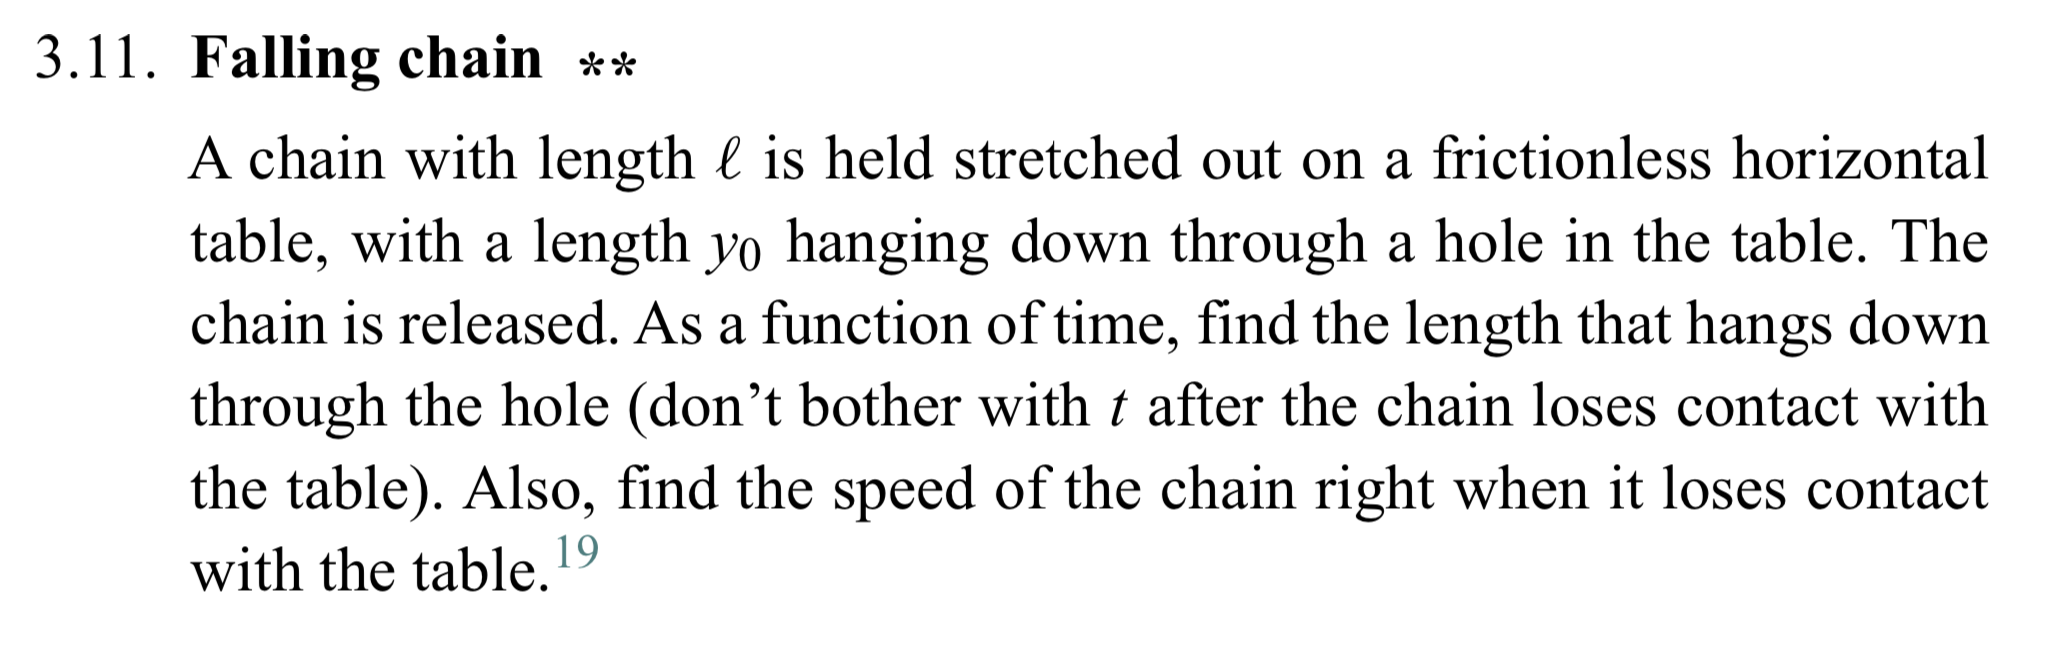
\includegraphics[width=400pt]{img/physics--classical-mechanics--morin--3-11.png}
\end{mdframed}

Let $y(t)$ be the length of chain hanging below the hole at time $t$, and let the density of the
chain be $\rho > 0$. From the Second Law we have
\begin{align*}
  l \rho \ddot{y} &= y\rho g \\
  \ddot{y} &= \frac{g}{l} y,
\end{align*}
Note that this is a second-order ODE and hence will have a 2-dimensional space of solutions. By
inspection, the space of solutions is $y(t) = Ae^{\alpha t} + Be^{-\alpha t}$, for real $A$, $B$,
where $\alpha = \sqrt{\frac{g}{l}}$.

The initial conditions yield
\begin{align*}
  y_0 &= A + B ~~~~~~~\text{from initial position}\\
  0   &= \alpha(A - B) ~~~~~~~\text{from initial velocity},
\end{align*}
therefore the solution is
$y(t) = \frac{y_0}{2}\(e^{\alpha t} + e^{-\alpha t}\) = y_0\cosh \alpha t$ (\red{\checkmark}), and
the velocity function is $\dot{y}(t) = y_0\alpha\sinh \alpha t$.

The chain loses contact with the table at time $t^*$ satisfying $\cosh \alpha t^* =
\frac{l}{y_0}$. Since $\sinh x = \sqrt{\cosh^2 x - 1}$, the velocity when the chain loses contact
with the table is
\begin{align*}
  y_0\alpha\sinh \alpha t^* = y_0\alpha\sqrt{\(\frac{l}{y_0}\)^2 - 1}.
\end{align*}




\subsection*{Projectile motion}
\subsection*{Motion in a plane, polar coordinates}
\subsubsection*{Example}
\begin{mdframed}
  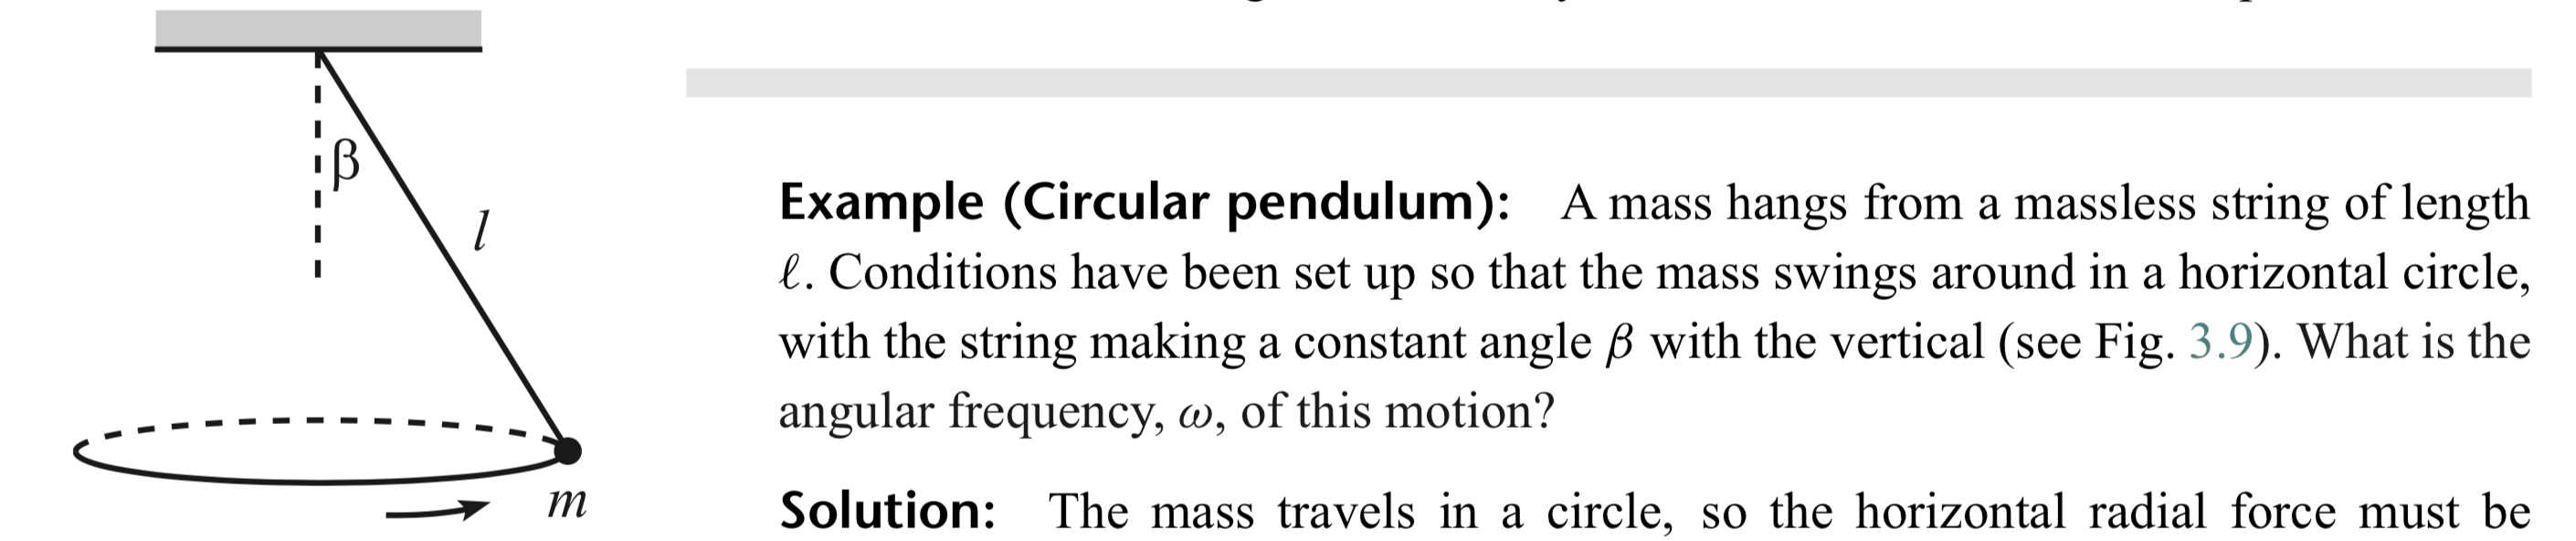
\includegraphics[width=400pt]{img/physics--classical-mechanics--morin--3--example-1.png}
\end{mdframed}

Fix a polar coordinate system for the plane of circular motion, such that $r = l\sin\beta$ is the
distance from the center and $\theta$ is the angle in radians relative to some $\theta=0$. The task
is to find $\dot{\theta}$.

Note that, since the units of $\theta$ are radians, by definition $r\theta$ is the position along
the circumference, and so $v = r\dot{\theta}$ is the the tangential velocity in the Cartesian
coordinate system.

Since the motion is circular, there must be a centripetal acceleration of magnitude
$v^2/r = r\dot{\theta}^2 = l\sin\beta\dot{\theta}^2$ directed radially towards the center.

Let $T$ be the string tension force. Since the mass is not accelerating vertically, we have that
$T\cos\beta = mg$.

The next step is to equate the centripetal acceleration with the net force that is causing it. This
force is the horizontal component of the string tension, i.e. $T\sin\beta = mg\tan\beta$.

Thus we have that $mg\tan\beta = ml\sin\beta\dot{\theta}^2$, and so the angular velocity is
$\omega = \dot{\theta} = \sqrt{\frac{g}{r\cos\beta}}$.

Checks:
\begin{itemize}
\item The units are $(LT^{-2}/L)^{1/2} = T^{-1}$. \checkmark
\item If the angle is to be larger, $\dot{\theta}$ must be faster. \checkmark
\item If the angle is to be constant, while gravity becomes stronger, $\dot{\theta}$ must be
  faster. \checkmark
\item If the angle is to be constant, while the radius becomes larger, $\dot{\theta}$ must be
  slower. \checkmark
\end{itemize}


\subsection*{3.20 Centripetal acceleration}
\begin{mdframed}
  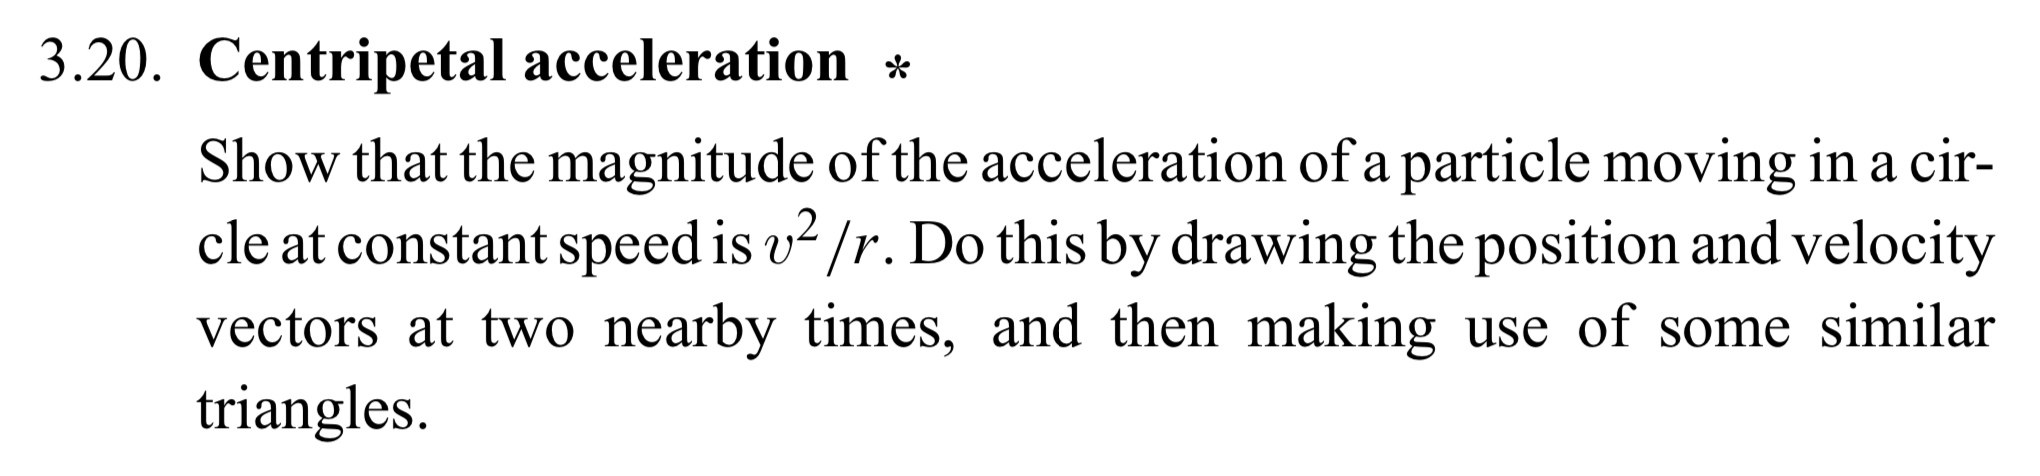
\includegraphics[width=400pt]{img/physics--classical-mechanics--morin--3-20.png}
\end{mdframed}

Suppose that a particle is moving in a circle at a constant speed of $v$ radians per second. At time
$t = 0$ its position vector is $\vec{r_1}$ and its velocity vector is $\vec{v_1}$, pointing
tangentially.  After $\Delta t$ seconds, its position vector is $\vec{r_2}$ and its velocity vector
is $\vec{v_2}$.

Define $\Delta \vec{r} = \vec{r_2} - \vec{r_1}$ and $\Delta \vec{v} = \vec{v_2} - \vec{v_1}$.  Note
that the angle between $\vec{v_1}$ and $\vec{v_2}$ is the same as that between $\vec{r_1}$ and
$\vec{r_2}$\footnote{According to the solutions in the book, this follows from the fact that the
  tangential velocity vectors are both perpendicular to their respective radial position
  vector.}. Therefore the triangle of position vectors, and velocity vectors are similar and we have
\begin{align*}
  \frac{|\Delta \vec{v}|}{v} &= \frac{|\Delta \vec{r}|}{r} \\
  \frac{|\Delta \vec{v}|}{\Delta t} &= \frac{v}{r}\frac{|\Delta \vec{r}|}{\Delta t} = \frac{v^2}{r},
\end{align*}
where $r = |\vec{r_1}| = |\vec{r_2}|$ and $v = |\vec{v_1}| = |\vec{v_2}|$.

{\bf Intuition:} The similar triangles argument says that the relationship between the second and
first derivatives parallels that between the first and zeroth derivatives:
\begin{align*}
  \frac{\ddot{\vec{r}}}{|\dot{\vec{r}}|} = \frac{\dot{\vec{r}}}{|\vec{r}|},
\end{align*}
from which $\ddot{r} = \frac{\dot{r}^2}{r}$ follows.


\subsubsection*{3.21 Vertical acceleration}
\begin{mdframed}
  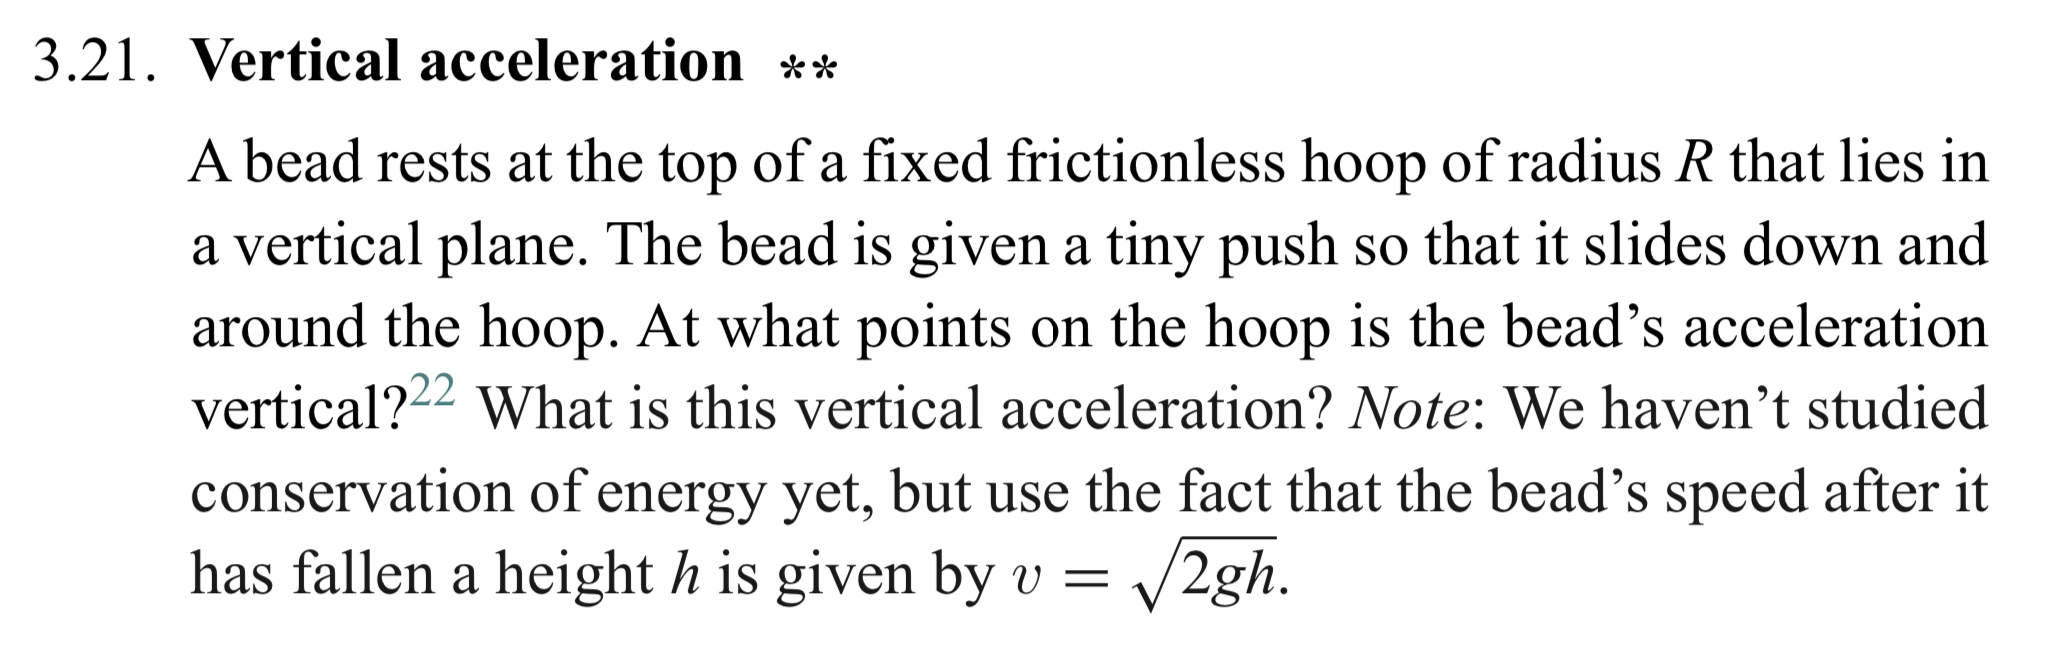
\includegraphics[width=400pt]{img/physics--classical-mechanics--morin--3-21.png}
\end{mdframed}

Let $\theta$ be the angle of the bead in radians measured clockwise from the top of the hoop.

When the bead has angle $\theta$, the weight has a radial component $g\cos\theta$ (opposed by an
equal normal reaction force) and a tangential component $g\sin\theta$ (unopposed). In addition,
there is a radial centripetal acceleration of magnitude $v^2/R$. The resultant acceleration will be
vertically downwards whenever the centripetal acceleration is equal to $g\cos\theta$ (because then
it is the same as the radial component of the weight, which we know yields vertically downwards
weight), and also when $\sin\theta=0$ (see diagram below). Using the fact, from conservation of
energy, that $v = \sqrt{2gh} = \sqrt{2g(R - R\cos\theta)}$, we have
\begin{align*}
  g\cos\theta  &= \frac{v^2}{R} =2g(1 - \cos\theta)\\
  \cos\theta &= \frac{2}{3},
\end{align*}
at which point the acceleration is $g$ vertically downwards.

\begin{mdframed}
  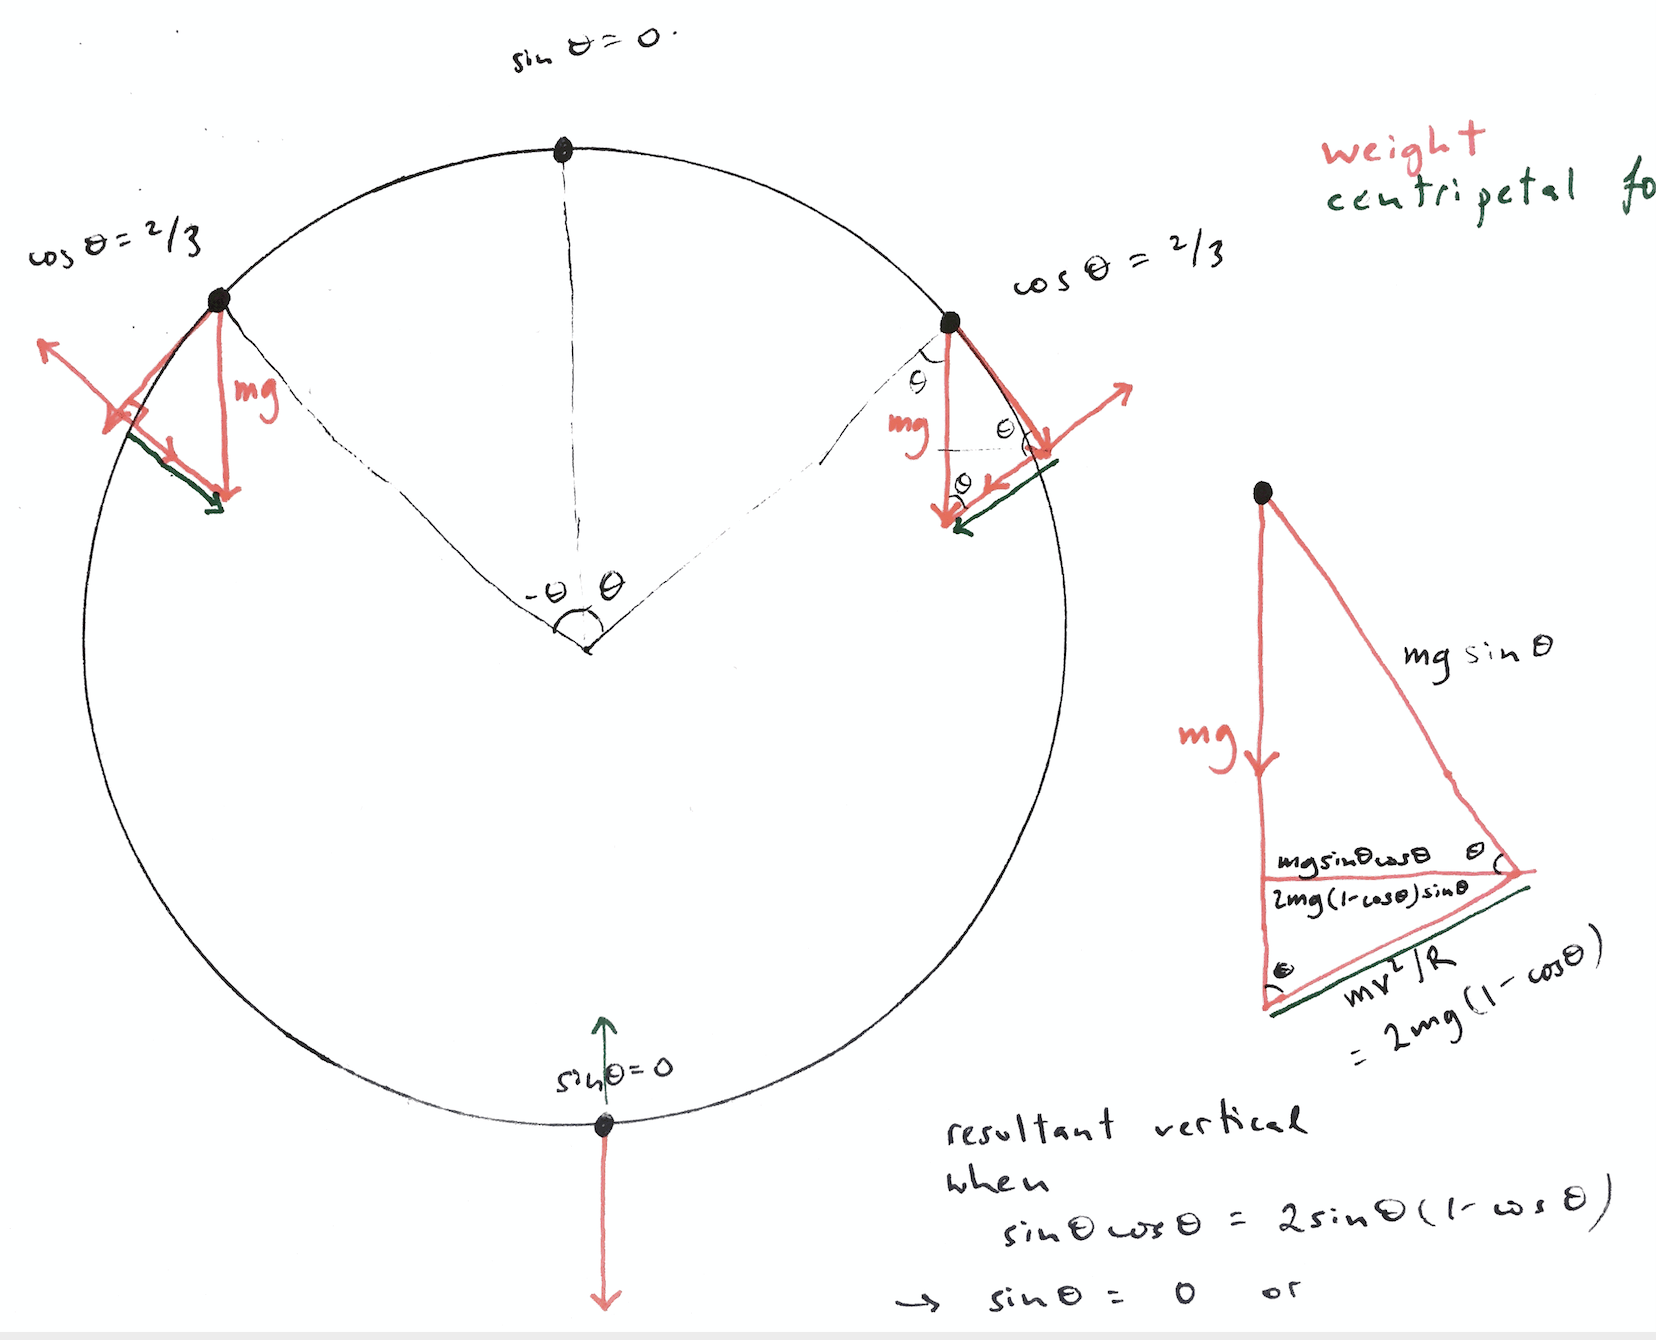
\includegraphics[width=300pt]{img/physics--classical-mechanics--morin--3-21-diag-2.png}
\end{mdframed}


\newpage
\subsubsection*{3.22 Circling around a pole}
\begin{mdframed}
  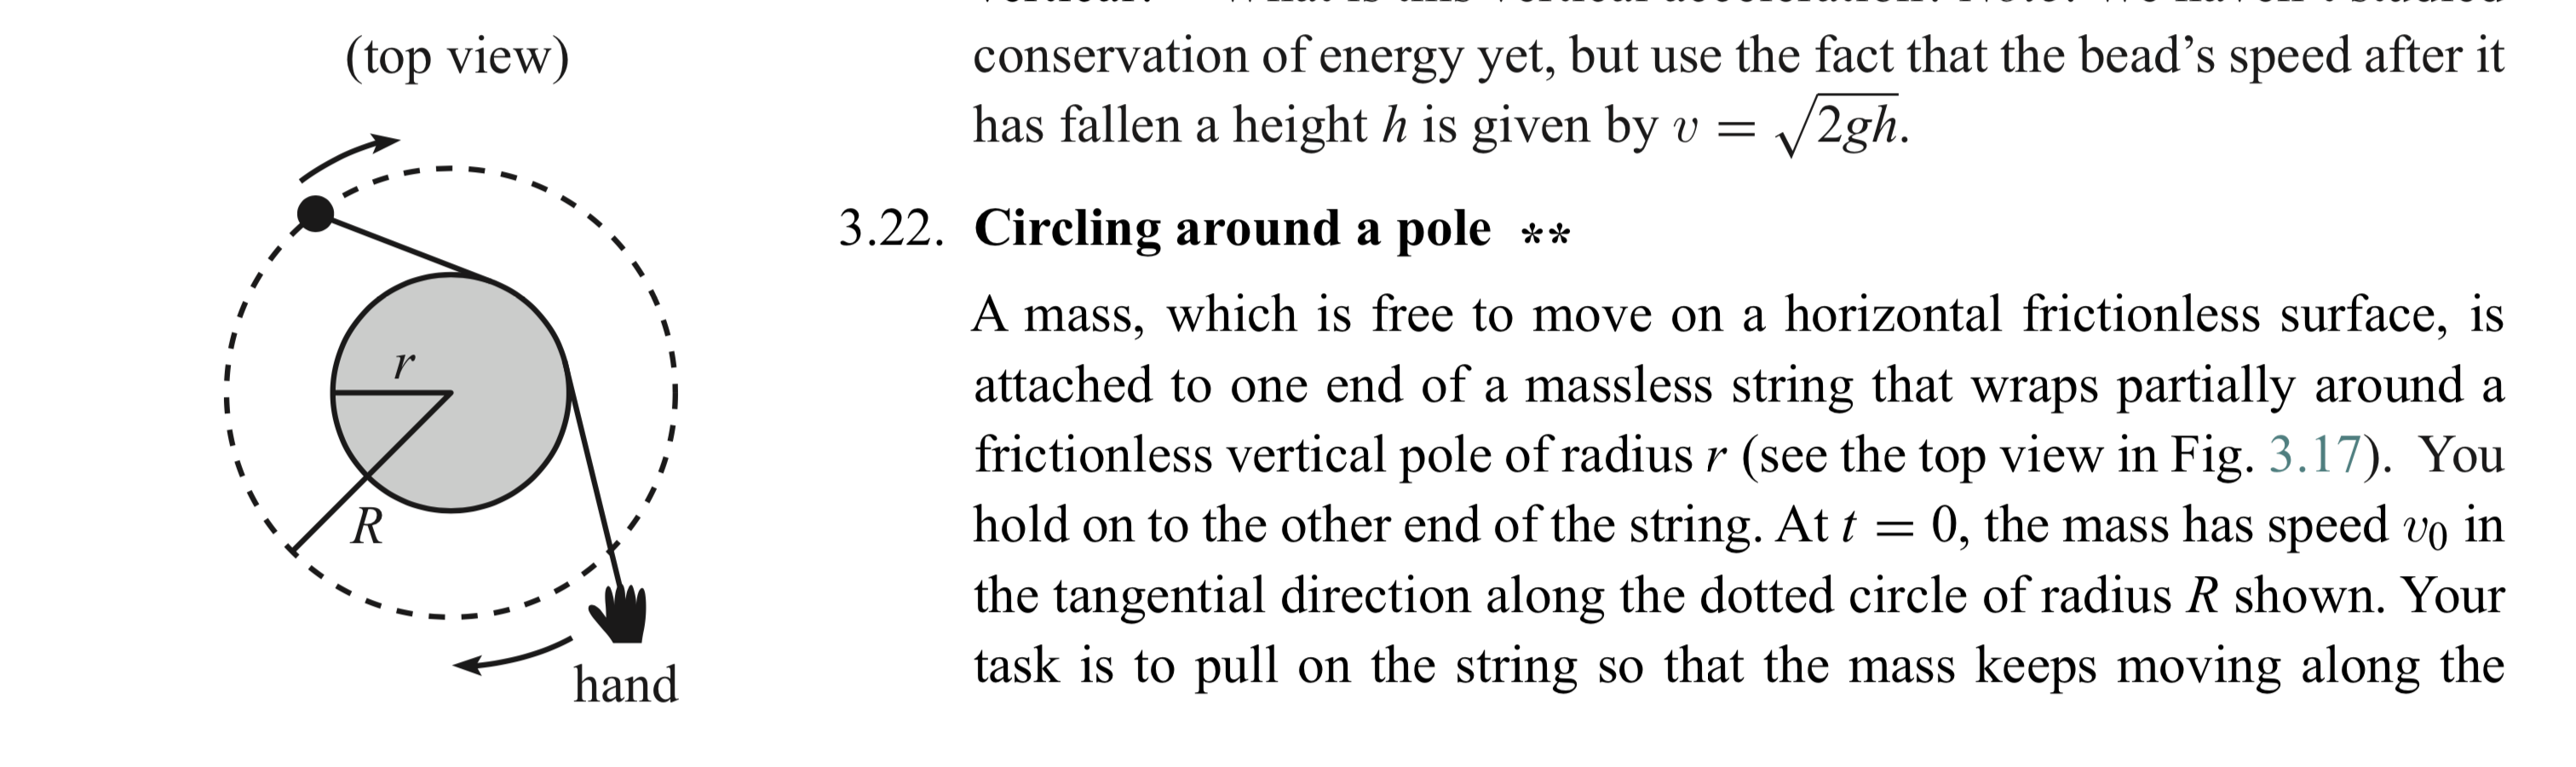
\includegraphics[width=400pt]{img/physics--classical-mechanics--morin--3-22.png}
\end{mdframed}
\begin{mdframed}
  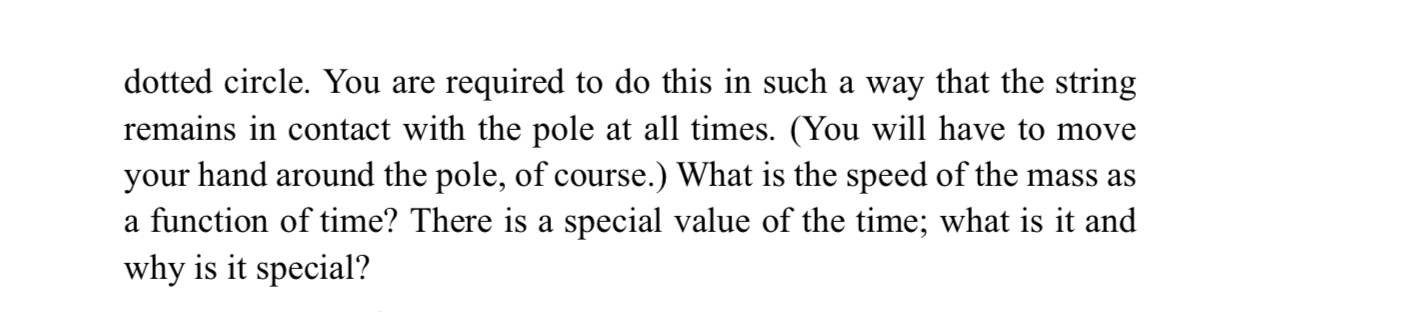
\includegraphics[width=400pt]{img/physics--classical-mechanics--morin--3-22-2.png}
\end{mdframed}




\section{Oscillations}





\section{Conservation of energy and momenum}
\subsection{Conservation of energy in one dimension}

\begin{enumerate}
\item Consider a force $F(x)$ that depends only on position. Then $E = T + V$ is constant over any
  trajectory resulting from that force under N2L.
\item $E$ and $V$ are defined in terms of an arbitrary starting point in space (and therefore
  initial velocity). But kinetic energy $T = E - V$ does not depend on the arbitrary start location.
\item Work-Energy theorem: change in $T$ equals work done.
\item $V$ may exceed $E$ in some regions of space; a N2L trajectory cannot enter such regions.
  \begin{mdframed}
    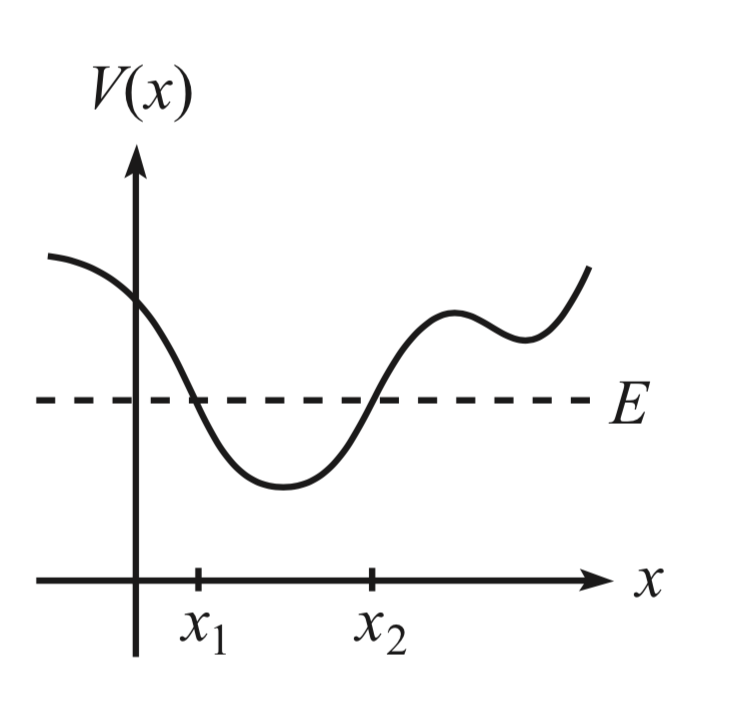
\includegraphics[width=100pt]{img/physics--classical-mechanics--morin--V-E-landscape.png}
  \end{mdframed}
\end{enumerate}

\subsubsection{Example: unwinding string}
A mass is connected to one end of a massless string, the other end of which is connected to a very
thin frictionless vertical pole. The string is initially wound completely around the pole, in a very
large number of tiny horizontal circles, so that the mass touches the pole. The mass is released,
and the string gradually unwinds. What angle does the string make with the pole at the moment it
becomes completely unwound?

\begin{proof}
  Let $m, l, \theta$ be the mass, the length of the string, and the final angle.

  When unwound, the mass has descended by $l\cos\theta$, so its potential energy has decreased by
  $mgl\cos\theta$. Let $v$ be its velocity at that point. Then
  \begin{align*}
    \frac{1}{2}mv^2 &= mgl\cos\theta\\
    v^2             &= 2gl\cos\theta.
  \end{align*}
  ...\red{incomplete}
\end{proof}

\subsubsection*{5.1}
\begin{mdframed}
  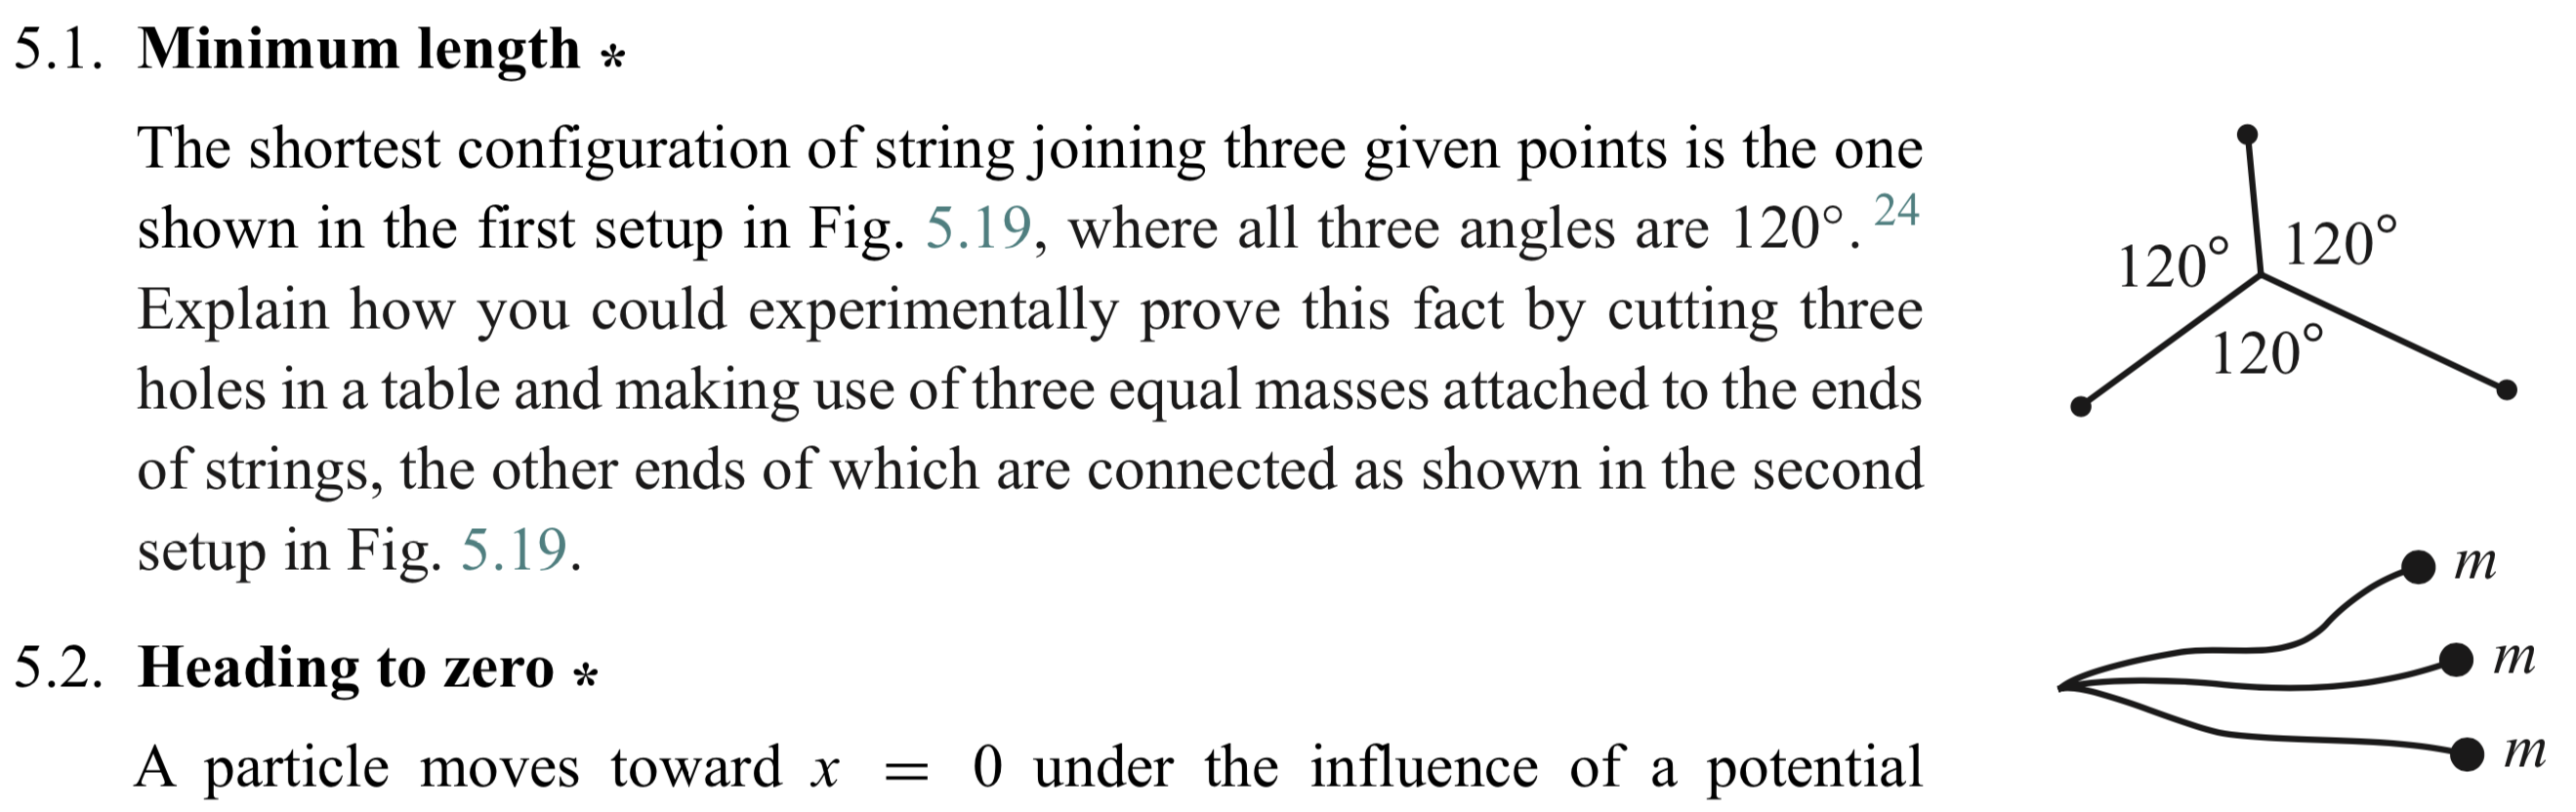
\includegraphics[width=400pt]{img/physics--classical-mechanics--morin--5-1.png}
\end{mdframed}

The masses will settle at their lowest potential energy. Suppose this were not a
minimum-string-above-table configuration. Then some mass would be able to descend, i.e. there would
be a force on the mass and it would descend. So the equilibrium configuration is a
minimum-string-above-table configuration.

Each mass pulls with an equal force $mg$, therefore the tension in each string is equal to
$mg$. These tensions at the central knot balance each other, since there is no motion. So
considering any one string, it must bisect the angle of the other two. Hence all 3 angles are equal,
and therefore equal to 120$\deg$.

\subsubsection*{5.2}
\begin{mdframed}
  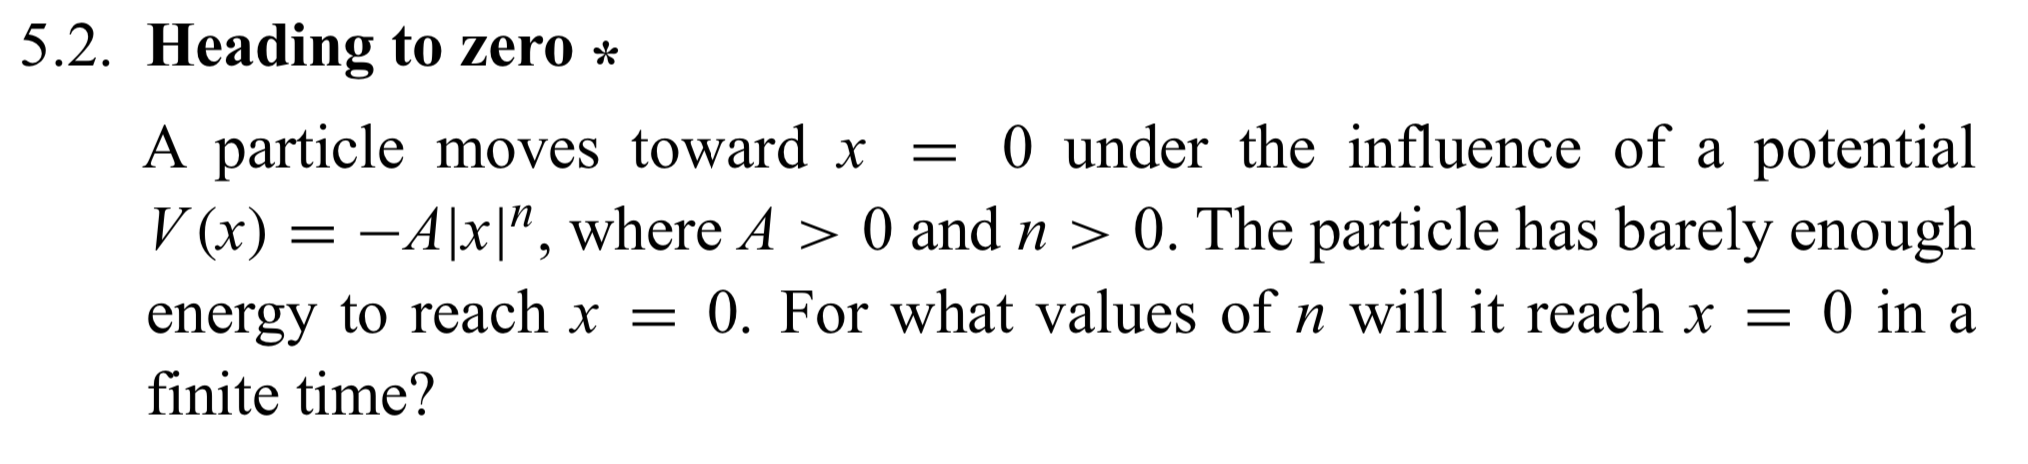
\includegraphics[width=400pt]{img/physics--classical-mechanics--morin--5-2.png}
\end{mdframed}

Let $T(x)$ be kinetic energy. The potential $V(x)$ is negative, increasing to $V(0) = 0$. At $x = 0$
the particle has no kinetic energy. Therefore the total energy is $T(x) + V(x) = 0$ and, measuring
$x$ in the direction of displacement of the particle, we have
\begin{align*}
  \frac{1}{2}mv^2 &= Ax^n \\
  v = \dxdt       &= a x^{n/2},
\end{align*}
where $a = \sqrt{2A/m}$. Separating variables, and letting $x_0$ be the starting position and $t$ be
the time taken to reach $x=0$, we have
\begin{align*}
  \int_{x_0}^0 x^{-n/2} \dx &= \int_0^t a\dt' = at.
\end{align*}
\todo{Don't think this is right:}
The antiderivative of $x^{-n/2}$ is $\frac{2}{2 - n}x^{-\frac{n - 2}{2}}$, which exists for
$n \neq 2$. Therefore these are the values of $n$ for which the particle reaches the origin in
finite time.

\subsubsection*{5.3}
\begin{mdframed}
  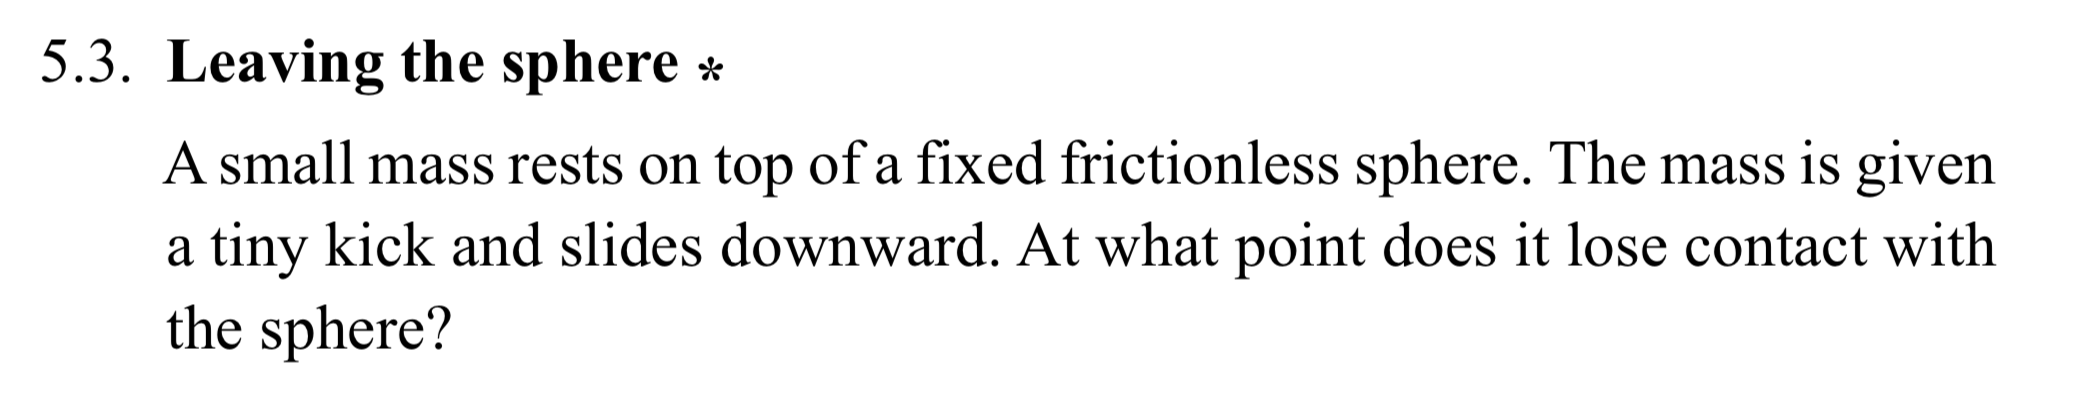
\includegraphics[width=400pt]{img/physics--classical-mechanics--morin--5-3.png}
\end{mdframed}

